
\documentclass[UTF8,a4paper,11pt]{ctexart}
\usepackage{geometry}
\geometry{left=2.5cm,right=2.5cm,top=2.6cm,bottom=2.6cm}
\usepackage{amsmath,amssymb,bm}
\usepackage{booktabs,longtable,tabularx,array,multirow}
\usepackage{enumitem}
\usepackage{graphicx}
\usepackage{xcolor}
\usepackage{hyperref}
\usepackage{titlesec}
\usepackage{fancyhdr}
\usepackage{tocloft}
\usepackage{caption}
\usepackage{float}
\usepackage{pdflscape}
\usepackage{url}
\hypersetup{colorlinks=true,linkcolor=blue,citecolor=blue,urlcolor=blue}
\setlist[itemize]{leftmargin=2em,itemsep=0.2em,topsep=0.2em}
\setlist[enumerate]{leftmargin=2.2em,itemsep=0.2em,topsep=0.2em}
\setlength{\headheight}{14pt}
\pagestyle{fancy}
\fancyhf{}
\lhead{FJSP 近五年研究综述}
\rhead{\thepage}
\renewcommand{\headrulewidth}{0.4pt}
\titleformat{\section}{\Large\bfseries}{\thesection}{0.8em}{}
\titleformat{\subsection}{\large\bfseries}{\thesubsection}{0.8em}{}
\titleformat{\subsubsection}{\normalsize\bfseries}{\thesubsubsection}{0.8em}{}
\newcommand{\fj}{\mathrm{FJSP}}
\newcommand{\Cmax}{C_{\max}}
\newcommand{\R}{\mathbb{R}}
\newcommand{\Z}{\mathbb{Z}}
\newcolumntype{Y}{>{\raggedright\arraybackslash}X}

\title{\bfseries 柔性作业车间调度问题（FJSP）研究综述\\[0.5em]
\large 从经典调度模型到智能、绿色与韧性制造的运筹学视角}
\author{匿名稿件}
\date{\today}

\begin{document}
\maketitle
\begin{abstract}
柔性作业车间调度问题（Flexible Job Shop Scheduling Problem, FJSP）是运筹学、组合优化与智能制造交叉领域中最具代表性的调度问题之一。与经典作业车间调度相比，FJSP 同时包含工序-机器分配、机器内排序与时间安排三类强耦合离散决策，因而既具有清晰的数学结构，又具有突出的工业应用价值。近年来，FJSP 研究已经从静态 makespan 最小化扩展到绿色低碳、动态扰动、分布式制造、AGV/机器人运输、预防性维护、工人柔性、多资源约束、韧性调度以及数字孪生驱动的实时优化等方向；求解技术也从混合整数规划、约束规划和经典元启发式，发展到自适应大邻域搜索、超启发式、强化学习辅助进化算法、图神经网络和深度强化学习等混合范式。本文按照“问题结构--模型扩展--算法谱系--应用闭环--实验规范--未来路线图”的逻辑，对近五年 FJSP 及其扩展问题进行系统性、批判性综述。不同于仅按年份或算法类型罗列文献的综述，本文强调统一数学结构、算法适用边界、结果可比性、实际落地条件和未来可验证研究命题，并对约百篇 FJSP 强相关文献逐类给出“问题设定、方法设计、主要贡献与局限”的细化评述。本文认为，未来高水平 FJSP 研究应从单纯追求启发式性能，转向“结构化优化模型、可验证求解器、学习型决策组件、标准化 benchmark 与工业数据闭环”的协同范式。
\end{abstract}

\noindent\textbf{关键词：}柔性作业车间调度；组合优化；混合整数规划；约束规划；元启发式；深度强化学习；图神经网络；绿色调度；动态调度

\vspace{0.8em}
\noindent\textbf{本文贡献：}本文的主要贡献包括四点：第一，提出覆盖问题设定、模型扩展、算法谱系、应用闭环和研究路线图的 FJSP 分类框架；第二，将 FJSP 的核心数学结构和主要扩展统一到工序-资源-时间网络中；第三，对精确算法、启发式、元启发式和学习型算法分别讨论适用条件、可扩展性和失效模式；第四，围绕绿色制造、韧性制造、AGV 运输、维护、数字孪生和多资源协同提出可验证的未来研究命题。

\tableofcontents
\newpage

\section{引言}

柔性作业车间调度问题（Flexible Job Shop Scheduling Problem, FJSP）是生产调度领域中最具代表性的组合优化问题之一。与经典 Job Shop Scheduling Problem (JSP) 相比，FJSP 允许一道工序在多台候选机器中选择其一完成，因此不仅要确定每台机器上的加工顺序，还要确定每道工序的机器分配。这个看似简单的扩展显著扩大了搜索空间，使 FJSP 同时包含路由选择、排序和时间安排三个层面的离散决策。

近年来，制造系统正在经历从传统车间到智能制造、绿色制造和韧性制造的转变。订单小批量、多品种、交货期紧张、设备状态不确定、能源价格波动和运输资源有限等因素，使得 FJSP 的研究不再局限于静态单目标 makespan 最小化。Dauz\`ere-P\'er\`es 等的综述指出，FJSP 已形成覆盖多目标、多约束、多配置和多算法范式的庞大研究体系\cite{Dauzere-Peres2024}。Li 等进一步从集成优化角度总结了 FJSP 与运输、维护、工人、装配等问题的耦合趋势\cite{Li2022SurveyIntegrated}。Destouet 等则将 FJSP 放在 Industry 5.0 语境下讨论，强调人本、环境和韧性三个维度\cite{Destouet2023Industry5}。

本文的目标不是简单罗列论文，而是回答三个问题：
\begin{enumerate}
    \item 近五年 FJSP 研究究竟围绕哪些问题设定和建模扩展展开？
    \item 精确算法、启发式、元启发式、学习型方法各自解决了什么痛点，又留下什么不足？
    \item 对于后续拟提出新方法的研究者，哪些方向更容易形成可投稿、可验证、可扩展的创新点？
\end{enumerate}


\section{可复现检索流程、元数据核验与文献计量分析}
\label{sec:protocol-bibliometrics}

为了使综述具备一区期刊所要求的透明性和可复核性，本文将文献整理过程显式化为四个阶段：检索、筛选、编码与核验。需要强调的是，本稿当前的统计分析基于已纳入的 $n=106$ 篇核心文献池，而不是声称穷尽 Scopus 或 Web of Science 中所有 FJSP 论文；正式投稿前，应进一步导出数据库检索记录并附录完整 PRISMA 流程图。

\subsection{检索数据库与检索式}

建议在正式版本中至少覆盖 Web of Science Core Collection、Scopus、ScienceDirect、IEEE Xplore、SpringerLink、ACM Digital Library、Wiley、Taylor \& Francis、MDPI、arXiv 与 Google Scholar。为保证可复现性，表\ref{tab:search-string} 给出可直接复用的检索式族。检索时间窗建议设为 1990--2026 年，其中近五年定义为 2021--2026 年；经典奠基文献不受时间窗限制。

\begin{table}[H]
\centering
\caption{FJSP 综述的可复现检索式族}
\label{tab:search-string}
\begin{tabularx}{\textwidth}{p{3.1cm}Y}
\toprule
检索目的 & 推荐检索式 \\
\midrule
核心问题 & \texttt{("flexible job shop" OR "flexible job-shop" OR FJSP OR FJSSP) AND scheduling} \\
绿色低碳 & \texttt{("flexible job shop" AND (energy OR green OR low-carbon OR carbon OR "time-of-use" OR "peak power"))} \\
动态与韧性 & \texttt{("flexible job shop" AND (dynamic OR rescheduling OR breakdown OR uncertain OR stochastic OR robust OR resilience))} \\
运输/AGV 集成 & \texttt{("flexible job shop" AND (AGV OR transport* OR crane OR vehicle OR robot OR logistics))} \\
多资源/维护 & \texttt{("flexible job shop" AND (maintenance OR worker OR operator OR "multi-resource" OR tool OR fixture OR buffer))} \\
学习型算法 & \texttt{("flexible job shop" AND ("reinforcement learning" OR "deep reinforcement" OR GNN OR "graph neural" OR transformer OR "machine learning"))} \\
\bottomrule
\end{tabularx}
\end{table}

\subsection{纳入与排除标准}

纳入标准包括：第一，题名、摘要或模型明确涉及 FJSP/FJSSP 或其直接扩展；第二，论文提出模型、算法、benchmark、应用案例或综述框架之一；第三，近五年文献优先，经典 benchmark 和奠基模型作为背景保留；第四，优先纳入期刊、重要会议、出版社正式页面可检索文献。排除标准包括：第一，仅讨论一般 JSP、flow shop 或 flexible flow shop 且无法映射到 FJSP 的文献；第二，仅有算法名称但缺少问题定义、约束和实验协议的弱相关文献；第三，题录信息无法核验且无可访问出版源的条目。

\subsection{元数据字段与核验规则}

每篇文献按如下字段编码：年份、问题类型、目标函数、约束扩展、算法家族、benchmark、是否有真实案例、是否开源、DOI 状态。DOI 被划分为三类：\emph{verified} 表示已从出版社页、Crossref 镜像、IEEE/MDPI/Springer/ScienceDirect/ACM 页面或可靠题录页确认；\emph{inferred-pattern} 表示 DOI 符合 Elsevier、MDPI 等 article-number 规则但本轮未逐页打开确认；\emph{unverified/no-doi} 表示暂未找到可靠 DOI 或条目本身为技术报告、预印本/early access。正式投稿时，后一类不应直接作为最终参考文献使用，而应进一步核验或替换。


\begin{table}[H]
\centering
\caption{当前文献池的元数据概况}
\label{tab:biblio-stats}
\begin{tabular}{lrr}
\toprule
指标 & 数量 & 占比 \\
\midrule
文献总数 & 106 & 100.0\% \\
2021--2026 年文献 & 96 & 90.6\% \\
已逐条加入 BibTeX 条目 & 106 & 100.0\% \\
DOI 已通过检索/出版社页核验 & 18 & 17.0\% \\
DOI 按出版社 article-number 规则推断，待正式复核 & 68 & 64.2\% \\
暂无可靠 DOI 或未完成核验 & 20 & 18.9\% \\
\bottomrule
\end{tabular}
\end{table}


\subsection{文献计量结果}

图\ref{fig:year-dist}--图\ref{fig:doi-status} 给出当前核心文献池的年度分布、主题分布、方法谱系分布和 DOI 核验状态。可以看到，2021 年以后 FJSP 文献明显向绿色低碳、动态韧性、运输/AGV 集成和学习型算法集中；与此同时，传统元启发式仍占较大比例，但越来越多论文将 Q-learning、深度强化学习、图神经网络或 ALNS/CP repair 嵌入元启发式框架中。该趋势表明，FJSP 研究正在从单一启发式改进转向“优化模型--学习组件--实时制造系统”的混合范式。

\begin{figure}[H]
\centering
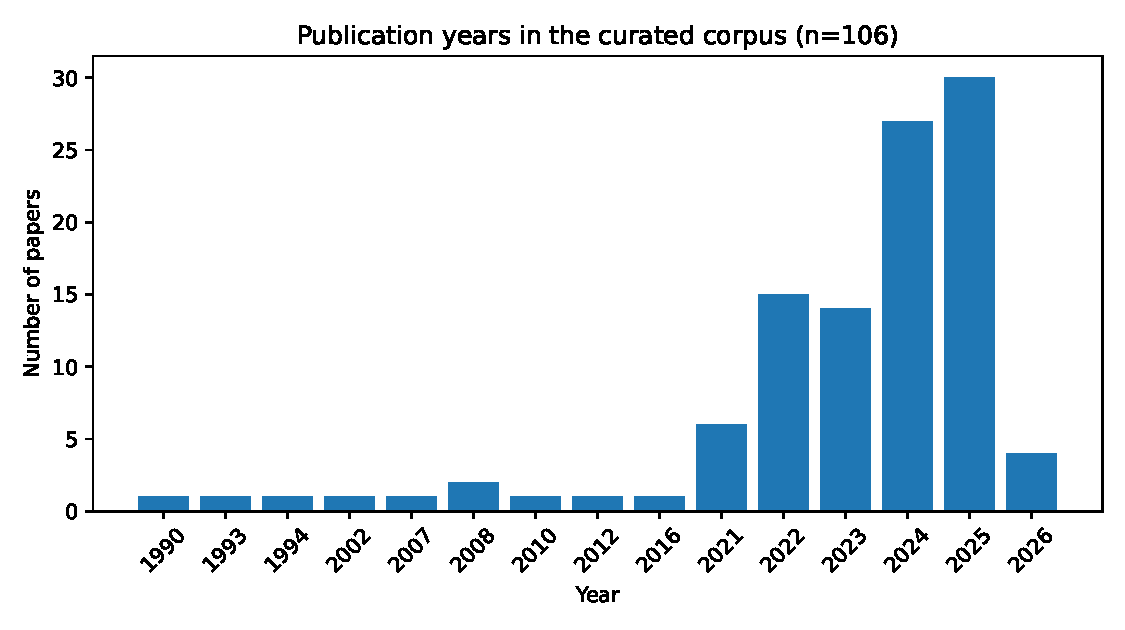
\includegraphics[width=0.82\textwidth]{fjsp_biblio_figures/year_distribution.pdf}
\caption{当前文献池按年份分布。}
\label{fig:year-dist}
\end{figure}

\begin{figure}[H]
\centering
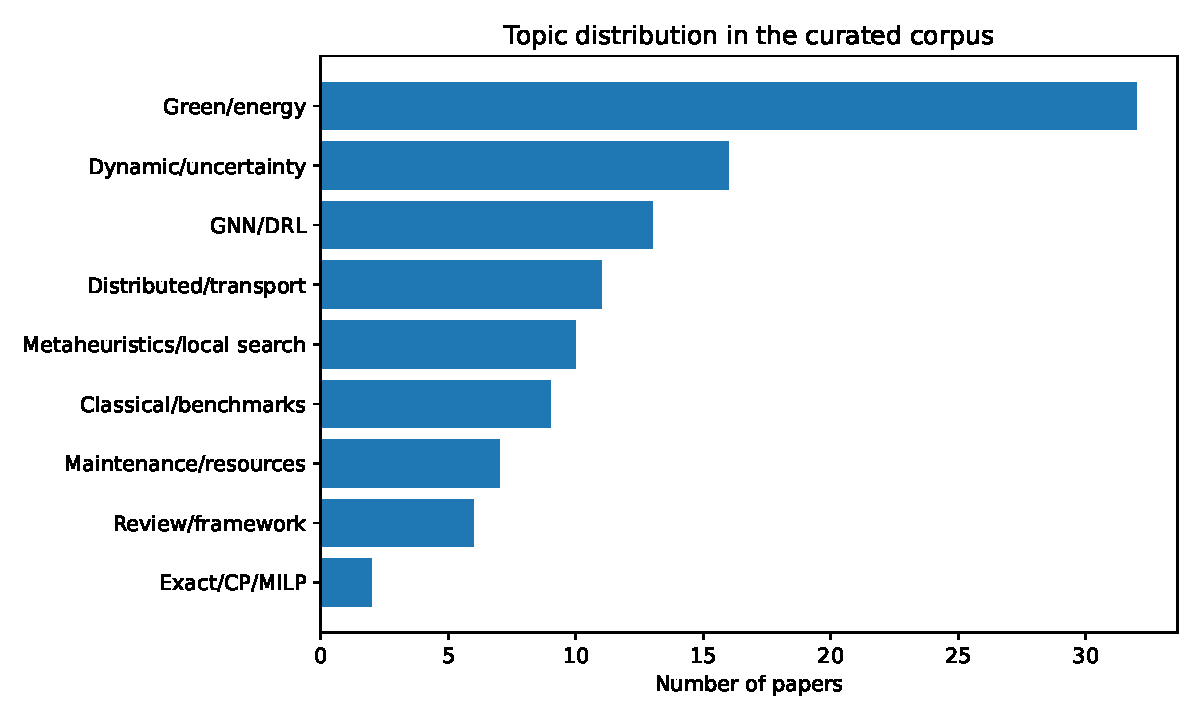
\includegraphics[width=0.88\textwidth]{fjsp_biblio_figures/theme_distribution.pdf}
\caption{当前文献池按主题分布。}
\label{fig:theme-dist}
\end{figure}

\begin{figure}[H]
\centering
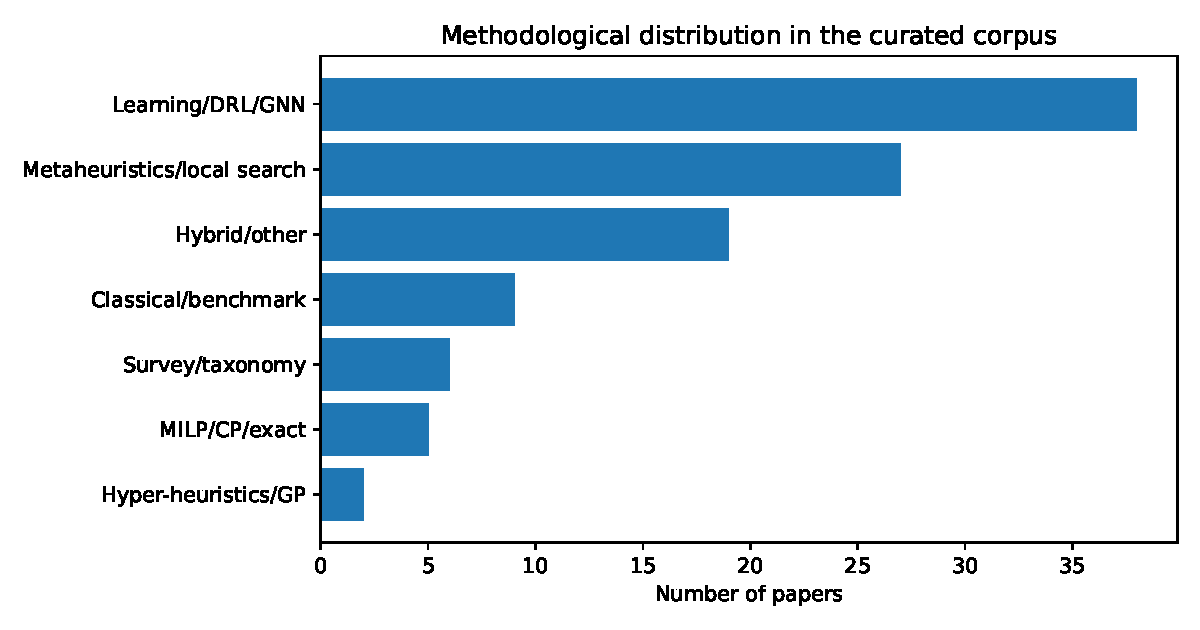
\includegraphics[width=0.88\textwidth]{fjsp_biblio_figures/method_distribution.pdf}
\caption{当前文献池按方法谱系分布。}
\label{fig:method-dist}
\end{figure}

\begin{figure}[H]
\centering
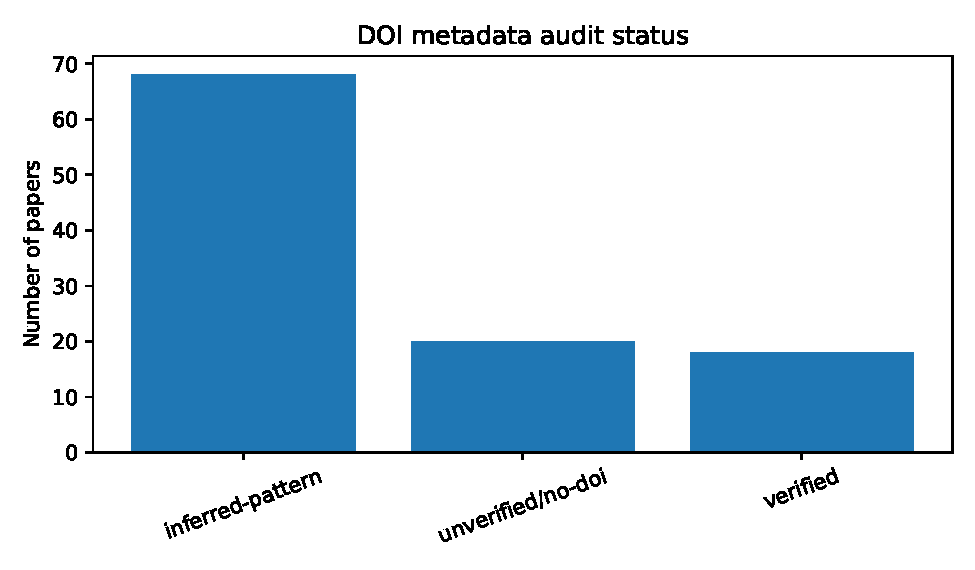
\includegraphics[width=0.68\textwidth]{fjsp_biblio_figures/doi_status.pdf}
\caption{当前文献池 DOI 元数据核验状态。}
\label{fig:doi-status}
\end{figure}

\subsection{对现有文献池的审稿式评价}

从一区综述标准看，当前文献池已经覆盖经典 FJSP、绿色低碳、动态调度、运输/AGV、维护、多资源和学习型调度等主线，但仍存在三个必须继续改进的问题。第一，若要进行真正的 bibliometric analysis，不能只统计人工纳入文献，而应从 Scopus/WoS 导出完整记录，报告检索日期、筛选数量、去重数量和排除原因。第二，当前不少 2025--2026 年条目属于 early access 或 article-in-press，正式投稿前必须逐条确认卷期页码、DOI 与出版状态。第三，算法比较不能只统计文献数量，还应进一步编码 benchmark、评价指标、是否开源、是否做统计显著性检验和是否报告运行时间。


\section{FJSP 问题定义与基本数学模型}

\subsection{基本对象}

设有工件集合 $J=\{1,2,\ldots,n\}$，机器集合 $M=\{1,2,\ldots,m\}$。每个工件 $j$ 包含 $n_j$ 道工序：
\[
J_j = \left(O_{j,1}, O_{j,2}, \ldots, O_{j,n_j}\right),
\]
且满足固定工艺顺序：
\[
O_{j,1}\rightarrow O_{j,2}\rightarrow \cdots \rightarrow O_{j,n_j}.
\]
对于每道工序 $O_{j,h}$，其候选机器集合记为 $M_{j,h}\subseteq M$。若 $k\in M_{j,h}$，则 $p_{j,h,k}$ 表示该工序在机器 $k$ 上的加工时间。

FJSP 的基本决策包括：
\begin{itemize}
    \item 机器选择：每道工序选择哪台可加工机器；
    \item 机器排序：同一台机器上多道工序按照什么顺序加工；
    \item 时间安排：每道工序何时开始、何时结束。
\end{itemize}

\subsection{经典 MILP 模型}

将所有工序集合记为 $O$。定义二进制变量：
\[
 x_{o,k}=\begin{cases}
1, & \text{工序 }o\text{ 被分配到机器 }k,\\
0, & \text{否则},
\end{cases}
\]
其中 $k\in M_o$。定义开始时间 $S_o\geq 0$、完工时间 $C_o\geq 0$，以及最大完工时间 $\Cmax$。对于共享候选机器 $k$ 的两道工序 $o,q$，定义排序变量：
\[
 y_{o,q,k}=\begin{cases}
1, & \text{若在机器 }k\text{ 上 }o\text{ 先于 }q,\\
0, & \text{若在机器 }k\text{ 上 }q\text{ 先于 }o.
\end{cases}
\]

以最小化最大完工时间为例，基本 MILP 可以写为：
\begin{align}
\min\quad & \Cmax \\
\text{s.t.}\quad
& \sum_{k\in M_o}x_{o,k}=1, && \forall o\in O, \\
& C_o = S_o + \sum_{k\in M_o}p_{o,k}x_{o,k}, && \forall o\in O,\\
& S_{j,h+1}\geq C_{j,h}, && \forall j\in J,\ h=1,\ldots,n_j-1,\\
& S_q \geq C_o - B(1-y_{o,q,k})-B(2-x_{o,k}-x_{q,k}), && \forall o<q,\ k\in M_o\cap M_q,\\
& S_o \geq C_q - By_{o,q,k}-B(2-x_{o,k}-x_{q,k}), && \forall o<q,\ k\in M_o\cap M_q,\\
& \Cmax\geq C_o, && \forall o\in O,\\
& x_{o,k}\in\{0,1\},\ y_{o,q,k}\in\{0,1\}, && \\
& S_o,C_o,\Cmax\geq 0. &&
\end{align}
其中 $B$ 是足够大的常数。该模型结构清晰，但排序变量和 Big-M 约束会快速膨胀，并造成线性松弛较弱的问题。

\subsection{CP/CP-SAT 建模思想}

约束规划（Constraint Programming, CP）通常比 MILP 更自然地表达调度问题。对于 FJSP，CP 模型常用：
\begin{itemize}
    \item interval variable 表示工序加工区间；
    \item optional interval 表示工序在某候选机器上的可选加工模式；
    \item exactly-one 约束表达机器选择；
    \item no-overlap 约束表达同一机器容量为 1；
    \item precedence 约束表达工件内部工艺顺序。
\end{itemize}
相比 MILP，CP 避免了大量 Big-M 非重叠约束，适合处理工艺约束、时间窗、维护窗口和多资源占用等约束；但当目标函数包含复杂线性成本、能耗、电价或碳排放时，MILP 与 CP 的混合建模往往更有优势。

\section{近五年研究主题分类}

近五年 FJSP 的研究可以按“问题扩展”和“求解技术”两个维度组织。表 \ref{tab:taxonomy} 给出一个简要分类。

\begin{table}[H]
\centering
\caption{近五年 FJSP 研究主题分类}
\label{tab:taxonomy}
\begin{tabularx}{\textwidth}{p{3.0cm}Y Y}
\toprule
类别 & 典型问题设定 & 代表性方法 \\
\midrule
经典静态 FJSP & makespan、机器负载、总完工时间 & MILP、CP、GA、TS、VNS、GNN-DRL \\
绿色/低碳 FJSP & 能耗、碳排放、峰值功率、TOU 电价、可变加工速度 & MOEA/D、NSGA-II/III、memetic algorithm、Q-learning EA \\
动态 FJSP & 新订单到达、机器故障、急单插入、加工时间扰动 & DRL、DQN/DDPG、重调度、GP 超启发式 \\
分布式 FJSP & 多工厂/多车间、订单分配、跨工厂运输 & 协同进化、分层编码、分布式 memetic algorithm \\
运输/AGV 集成 FJSP & 机器与运输资源联合调度、AGV 路径与车辆选择 & MILP+GA、ALNS、quality-diversity、DRL \\
维护集成 FJSP & 固定/周期预防性维护、退化、随机故障 & MILP、CP、协同局部搜索、鲁棒优化 \\
人本/多资源 FJSP & 工人柔性、工人班次、技能、疲劳、工具夹具资源 & 统一多资源建模、CP、ALNS、双资源调度 \\
学习型 FJSP & 学习派工规则、学习邻域、端到端调度策略 & GNN、HGNN、Transformer、DRL、MARL \\
\bottomrule
\end{tabularx}
\end{table}

\section{精确算法、数学规划与约束规划}

\subsection{MILP 及其适用边界}

MILP 是 FJSP 最标准的可验证建模方式，尤其适合小规模实例、基准验证和作为 matheuristic 中的 repair 子问题。Özgüven 等较早系统讨论了具有路由和工艺计划柔性的作业车间数学模型\cite{Ozgüven2010}。近五年，MILP 更常出现在扩展问题中，例如可控加工时间与能耗权衡\cite{Meng2023CPT}、预防性维护\cite{Zhao2025MILPPM}、AGV 集成\cite{Han2024AGV}、序列柔性\cite{Tang2024DFJSP}等。

MILP 的主要优点是：
\begin{enumerate}
    \item 模型表达精确，便于给出最优性证明和下界；
    \item 便于处理线性成本，如能耗、电价、碳排放、延迟罚金；
    \item 可作为启发式/学习算法的验证器或局部优化器。
\end{enumerate}

不足也很明显：
\begin{enumerate}
    \item Big-M 非重叠约束导致 LP 松弛弱；
    \item 排序变量数量随工序对和候选机器交集迅速增长；
    \item 对大规模动态实例难以实时求解。
\end{enumerate}

\subsection{CP 与 CP-assisted metaheuristic}

CP 使用区间变量和 no-overlap 约束直接表达机器容量约束，近年来在复杂约束 FJSP 中再次受到重视。Boyer 等在广义 FJSP 中同时提出 CP 与 MIP 模型，并加入最大时间间隔、holding time、机器容量和 sequence-dependent setup time 等约束\cite{Boyer2021GFJSP}。Zhao 等针对带预防性维护的 FJSP 构造 CP 模型，并进一步设计 CP-assisted 元启发式\cite{Zhao2025CPPM}。Kasapidis 等提出多资源约束 FJSP 的统一框架，说明 CP/ALNS-CP 对资源约束扩展具有较好适配性\cite{Kasapidis2025Unified}。

从方法论上看，CP 在 FJSP 中有三种价值：
\begin{itemize}
    \item 作为小规模最优求解器，给启发式和学习型方法提供 benchmark；
    \item 作为局部修复器，在 ALNS/LNS 中修复被破坏的子问题；
    \item 作为可行性检查器，用于过滤 LLM/RL/EA 生成的候选调度。
\end{itemize}

\section{启发式、派工规则与瓶颈思想}

\subsection{派工规则}

派工规则（dispatching rules）是最早、最简单、也最适合在线调度的一类方法。常见规则包括 SPT、LPT、MWKR、MOPNR、EDD、CR、FIFO、LWL 和 ECT 等。对于 FJSP，派工规则通常分两层：先选择就绪工序，再选择机器。例如，MWKR+ECT 会优先调度剩余工作量最大的工件，并把工序分配到最早完工的机器上。

派工规则的优势是极快、易实现、可解释，适合动态车间事件驱动决策。缺点是局部短视，无法稳定处理复杂耦合约束。因此近五年很多研究不再手工固定单一规则，而是通过强化学习、遗传规划或超启发式在不同规则之间自适应切换。例如动态 FJSP 中的 DQN/DDPG 类方法往往把若干 dispatching rules 作为动作空间，或学习一组规则权重\cite{Gui2023DDPG,Wang2022MORL}。

\subsection{Shifting Bottleneck 与关键路径邻域}

Shifting Bottleneck 最早用于 JSP，其基本思想是逐步识别瓶颈机器并确定该机器上的排序。在 FJSP 中，该思想通常需要与机器选择、局部搜索或 LNS 结合：先给工序分配机器，然后在关键机器或关键路径上进行排序优化。虽然近五年直接以 shifting bottleneck 为核心的 FJSP 论文不如 GA/DRL 多，但“瓶颈机器”“关键路径”“关键块”仍然是大量元启发式和邻域搜索设计的基础。

一个具有研究价值的方向是将瓶颈思想转化为可学习的 destroy/repair 策略：例如优先破坏关键路径上的工序、负载最高的机器、能耗峰值时段或维护窗口附近的工序，再用 CP/MILP 修复。

\section{元启发式与学习辅助进化算法}

\subsection{传统元启发式}

FJSP 的经典元启发式包括遗传算法、禁忌搜索、模拟退火、粒子群、蚁群、人工蜂群、差分进化、变邻域搜索和 memetic algorithm。传统双层编码 $(MS,OS)$ 仍是主流：$MS$ 表示机器选择，$OS$ 表示工序排序。Pezzella 等、Gao 等和 Brandimarte 等奠定了 FJSP 元启发式编码与搜索的基础\cite{Brandimarte1993,Pezzella2008,Gao2008}。

近五年中，单纯“改进某个自然启发式算法”的论文仍然很多，但高质量工作通常不再只停留在算子层面，而是同时强调：
\begin{itemize}
    \item 针对 FJSP 结构设计编码与解码；
    \item 引入关键路径、瓶颈机器或负载平衡的局部搜索；
    \item 面向多目标构建非支配排序、参考向量或分解机制；
    \item 用 Q-learning/RL 自适应选择邻域、算子或参数。
\end{itemize}

例如 Sun 等将遗传算法与变邻域搜索结合用于加工系统 FJSP\cite{Sun2023HGA}；Tang 等针对分布式 FJSP 与集成序列柔性设计 memetic algorithm\cite{Tang2024DFJSP}；Xie 等将遗传算法与禁忌搜索结合用于分布式 FJSP\cite{Xie2023HGTS}。

\subsection{超启发式与强化学习辅助元启发式}

超启发式的目标不是直接搜索调度解，而是搜索“如何选择启发式”。在 FJSP 中，超启发式可以选择：
\begin{itemize}
    \item 当前使用哪条派工规则；
    \item 当前执行哪种邻域；
    \item 采用哪种交叉、变异、局部搜索算子；
    \item 什么时候强化搜索、什么时候扩大多样性。
\end{itemize}

Zhang 等提出 Q-learning-based hyper-heuristic evolutionary algorithm 来求解带桥式起重机运输的分布式 FJSP\cite{Zhang2023CraneQL}。Zhang 等又将强化学习嵌入能耗感知 FJSP 的进化算法中\cite{Zhang2024EATA}。这类方法对于未来研究很重要，因为它们在“启发式可解释性”和“学习自适应性”之间形成了折中。

\section{绿色、低碳与能耗感知 FJSP}

\subsection{目标函数扩展}

绿色 FJSP 是近五年最活跃的方向之一。常见目标包括：
\[
\min \Cmax,\quad \min TEC,\quad \min TCE,\quad \min TWT,\quad \min P_{peak},
\]
其中 $TEC$ 表示总能耗，$TCE$ 表示总碳排放，$TWT$ 表示总加权拖期，$P_{peak}$ 表示峰值功率。能耗建模通常区分：
\begin{itemize}
    \item 加工能耗；
    \item 待机/空闲能耗；
    \item 开机/关机/重启能耗；
    \item 运输能耗；
    \item 不同加工速度下的能耗；
    \item 分时电价或需求响应下的能源成本。
\end{itemize}

Park 等研究 TOU 电价和计划停机下的能耗感知 FJSP\cite{Park2022TOU}；Wang 等研究低碳 many-objective FJSP，并提出改进 MOEA/D\cite{Wang2024MOEAD}；Wang 等考虑峰值功率约束、setup 和运输时间\cite{Wang2024PeakPower}；Zhao 等研究能效鲁棒 FJSP 并引入 DQL-assisted competitive evolutionary algorithm\cite{Zhao2024ERFJSP}。

\subsection{绿色 FJSP 的研究趋势}

绿色 FJSP 的关键趋势包括：
\begin{enumerate}
    \item 从单纯能耗最小化转向生产效率、能耗、碳排放、稳定性和鲁棒性的多目标权衡；
    \item 从固定加工速度转向 variable processing speed；
    \item 从单车间转向 distributed green FJSP；
    \item 从静态能耗转向动态电价、需求响应和可再生能源驱动；
    \item 从单一机器能耗转向机器、AGV、工人、维护和库存的综合能耗。
\end{enumerate}

对于方法创新而言，绿色 FJSP 的挑战在于目标函数复杂且约束强耦合：调度方案可能降低 makespan，却增加峰值功率；也可能降低能耗，却导致拖期增加。因此，多目标求解、Pareto 前沿质量、决策偏好注入和可解释 trade-off 分析都非常重要。

\section{动态 FJSP、不确定性与重调度}

动态 FJSP 研究的出发点是静态调度方案在真实车间中经常失效。常见扰动包括机器故障、新订单到达、急单插入、加工时间变化、运输资源不足、工人缺勤和维护事件。动态问题通常采用两种范式：
\begin{itemize}
    \item 事件驱动重调度：扰动发生后重新优化部分或全部调度；
    \item 在线调度：在每个决策点选择下一步动作，直接形成实时策略。
\end{itemize}

Luo 等较早将 DRL 用于动态多目标 FJSP\cite{Luo2021DRL}。Gui 等使用深度强化学习解决动态 FJSP\cite{Gui2023DDPG}。Zhang 等研究运输资源不足情形下的动态 FJSP，并使用深度 Q 网络学习优先规则\cite{Zhang2023InsufficientTR}。Fan 等考虑随机机器故障\cite{Fan2024Breakdown}。Li 等将知识引导的进化算法与强化学习结合，用于机器故障下的能效动态 FJSP\cite{Li2025KEARL}。

动态 FJSP 的评价指标不应只看最终 makespan，还应考虑：
\begin{itemize}
    \item 调度稳定性，即新旧调度变化幅度；
    \item 重调度计算时间；
    \item 平均拖期或加权拖期；
    \item 机器利用率和关键机器负载；
    \item 对未来扰动的鲁棒性。
\end{itemize}

\section{分布式、运输、AGV 与多资源 FJSP}

\subsection{分布式 FJSP}

分布式 FJSP（Distributed FJSP, DFJSP）考虑多个工厂或车间，除工序排序和机器选择外，还需要决定工件/订单分配到哪个工厂。该问题进一步扩大了搜索空间。近年来，DFJSP 常与能耗、运输、维护和序列柔性同时建模。例如 Tang 等考虑集成序列柔性的分布式 FJSP，并优化 makespan 与总能耗\cite{Tang2024DFJSP}；Zhang 等提出能耗感知分布式 FJSP 的概率模型进化算法\cite{Zhang2024ProbModel}；Zhou 等使用 DRL-based memetic algorithm 求解带有限运输资源的动态分布式绿色 FJSP\cite{Zhou2025DRLMA}。

\subsection{运输与 AGV 集成}

在真实车间中，工件从一台机器转移到另一台机器往往需要 AGV、起重机、移动机器人或人工搬运。Berterotti\`ere 等研究显式考虑运输资源的 FJSP，并扩展析取图来描述机器与运输操作\cite{Berterottiere2024Transport}。Han 等提出带 AGV 的 FJSP MILP 模型和双种群协同遗传算法\cite{Han2024AGV}。Li 等研究桥式起重机运输下的 FJSP\cite{Li2022Crane}。Qin 等进一步将 quality-diversity 与强化学习结合用于运输约束 FJSP\cite{Qin2025QD,Qin2026QDReal}。

这一方向的难点在于机器与运输资源之间存在同步关系：工序完成后，如果运输资源不可用，则下一道工序无法开始；反之，过早运输可能造成缓冲区占用和等待。因此，运输集成 FJSP 往往比普通 FJSP 更适合采用事件驱动仿真、CP/LNS 或多智能体强化学习。

\section{预防性维护、设备退化与鲁棒 FJSP}

预防性维护与 FJSP 的集成研究关注机器在生产过程中的可用性、维护窗口和故障风险。维护可以是固定窗口，也可以是周期性或状态依赖型。若调度忽略维护，所得方案可能在实际执行中不可行；若维护过于保守，则会降低设备利用率。

Wocker 等研究考虑预防性维护的 FJSP\cite{Wocker2024PM}。Wang 等研究高频生产切换下 FJSP 与预防性维护的联合优化\cite{Wang2024PM}。Zhao 等分别提出 MILP 和 CP 模型处理 FJSP-PM\cite{Zhao2025MILPPM,Zhao2025CPPM}。这些工作说明，维护集成 FJSP 具有很强的工业现实意义，也适合作为 solver-in-the-loop 框架的应用场景。

鲁棒 FJSP 进一步考虑扰动下的方案稳定性。典型策略包括：
\begin{itemize}
    \item 保留时间缓冲；
    \item 选择故障风险较低的机器；
    \item 优化可恢复性或重调度代价；
    \item 构造两阶段或多阶段鲁棒优化模型。
\end{itemize}

\section{GNN、DRL 与学习型 FJSP}

\subsection{为什么 FJSP 适合图表示}

FJSP 天然可以表示为图：工序是节点，工艺先后关系是有向边，候选机器关系是二部图边，机器冲突关系是析取边。与手工特征相比，图神经网络可以在调度状态中自动聚合：
\begin{itemize}
    \item 工序前驱/后继信息；
    \item 机器负载和空闲时间；
    \item 候选机器加工时间；
    \item 工件剩余工作量；
    \item 局部冲突和全局瓶颈。
\end{itemize}

Song 等提出基于 GNN 与 DRL 的 FJSP 求解框架，将工序选择与机器分配组合成复合决策\cite{Song2022GNNDRL}。Lei 等提出 multi-action DRL 框架，用 GNN 学习端到端调度策略\cite{Lei2022MultiAction}。Wan 等采用 meta-path-based heterogeneous GNN 处理 operation 和 machine 的异构关系\cite{Wan2024MHGNN}。Liu 等在 2025 年进一步使用图注意力网络从析取图中提取信息，构建端到端 DRL 框架\cite{Liu2025GNN}。

\subsection{DRL 方法的主要范式}

当前学习型 FJSP 大致分为三类：
\begin{enumerate}
    \item \textbf{学习派工规则选择：}动作是若干手工规则或规则权重，优点是稳定、可解释，缺点是策略空间有限。
    \item \textbf{端到端工序-机器选择：}动作直接是 $(operation,machine)$，表达能力强，但动作空间大、训练困难。
    \item \textbf{学习辅助优化：}DRL 不直接输出完整调度，而是选择邻域、算子、破坏/修复策略或 EA 参数。
\end{enumerate}

从研究趋势看，单纯端到端 DRL 虽速度快，但在解质量、最优性证明和跨规模泛化方面仍有不足。更有前景的方向可能是：
\[
\text{GNN/DRL 初始解或算子选择} + \text{CP/MILP/LNS 可验证改进}.
\]
这类 solver-in-the-loop 结构能够同时利用学习方法的速度与求解器的可行性保障。

\section{Benchmark、评价指标与实验设计}

\subsection{常用数据集}

FJSP 常用 benchmark 包括 Brandimarte MK、Hurink、Dauz\`ere-P\'er\`es、Kacem、Fattahi、Behnke-Geiger work center instances 等。对于扩展问题，研究者通常在这些 benchmark 上增加能耗参数、运输时间、AGV 数量、维护窗口、故障分布或动态订单到达机制。

实验设计中应避免只在自造实例上测试。更合理的基准组合包括：
\begin{itemize}
    \item 经典 FJSP benchmark：用于与传统算法比较；
    \item 中大规模随机实例：测试扩展性；
    \item 扩展场景实例：例如 AGV、energy、dynamic、maintenance；
    \item 小规模实例：用 MILP/CP 求最优，检验 optimality gap；
    \item 跨规模/跨分布测试：检验学习算法泛化。
\end{itemize}

\subsection{评价指标}

除了 $\Cmax$，近五年研究常用指标包括：
\begin{itemize}
    \item 总能耗 $TEC$、碳排放 $TCE$；
    \item 总拖期 $TT$、总加权拖期 $TWT$；
    \item 机器最大负载和总负载；
    \item AGV 总运输时间、等待时间和利用率；
    \item Pareto 前沿的 HV、IGD、Spread；
    \item 算法运行时间、稳定性和可扩展性；
    \item 动态环境中的平均响应时间和重调度扰动。
\end{itemize}

\section{现有研究不足}

\subsection{方法创新常停留在算子层面}

许多元启发式论文采用“改进 GA/PSO/ABC/DE”的形式，但创新点主要集中于交叉、变异、初始化、参数自适应等局部算子，缺少对 FJSP 结构本身的深入利用。未来更有价值的创新应当围绕关键路径、瓶颈机器、多资源冲突、能耗峰值和动态扰动机制构建结构化搜索。

\subsection{学习型方法泛化和可验证性不足}

DRL/GNN 方法通常在特定实例分布和规模上训练。一旦机器数、工件数、工序候选机器数、目标函数或约束类型发生变化，策略可能显著退化。此外，学习型方法很难给出最优性 gap 或可行性证明。因此，将学习策略与 CP/MILP/LNS 结合，是提高可信度的重要方向。

\subsection{Benchmark 不统一}

经典 FJSP benchmark 相对成熟，但绿色、AGV、维护、动态和分布式 FJSP 的实例生成协议并不统一。不同论文的能耗参数、AGV 速度、维护窗口、故障分布和电价曲线差异较大，导致算法横向比较困难。

\subsection{工业约束真实但理论解释不足}

近五年大量论文把 FJSP 扩展到真实制造约束，但理论分析相对不足。例如：为什么某种邻域对某类实例有效？为什么某种图表示具有跨规模泛化能力？如何解释学习到的派工策略？这些问题仍有较大研究空间。

\section{潜在研究方向与选题建议}

结合上述文献，可以考虑以下方向作为后续博士课题或论文投稿切入点。

\subsection{方向一：结构感知 LNS/ALNS for FJSP}

设计围绕 FJSP 结构的 destroy/repair 算子：
\begin{itemize}
    \item 关键路径 destroy；
    \item 瓶颈机器 destroy；
    \item 能耗峰值时段 destroy；
    \item AGV 等待链 destroy；
    \item 维护窗口附近 destroy；
    \item 多资源冲突 destroy。
\end{itemize}
修复阶段可以调用 CP、MILP 或轻量启发式，从而形成可验证的混合框架。

\subsection{方向二：LLM + 可验证优化 evaluator}

可以让 LLM 生成候选邻域、派工规则、破坏-修复策略或问题特定启发式，再由 optimisation evaluator 检查可行性、目标值和泛化性能。该方向的关键不是让 LLM 直接求解 FJSP，而是让 LLM 参与算法设计，并通过 CP/MILP/仿真器进行闭环验证。

\subsection{方向三：GNN-RL + Solver-in-the-loop}

GNN-RL 负责快速生成初始解、调度优先级或邻域选择；CP/MILP/LNS 负责局部修复和可验证优化。这一方向可以缓解纯 DRL 解质量不足和纯 solver 速度慢的问题。

\subsection{方向四：面向扩展 FJSP 的统一 DSL}

许多 FJSP 变体都可以抽象成：工序、资源、模式、 precedence、capacity、transition、calendar、energy、event。构建一个调度 DSL，把不同变体统一为可组合模块，再自动生成 CP/MILP/仿真环境，将非常适合与 LLM4Opt、algorithm unrolling 或自动算法设计结合。



\section{系统性文献筛选与评价框架}

系统性综述不能仅依赖作者主观挑选文献，而应明确说明文献筛选逻辑、纳入排除标准以及评价维度。FJSP 文献数量庞大，且许多论文题名相似、算法改名频繁，若不建立系统评价框架，容易形成“文献堆砌”。本文建议将 FJSP 文献评价分为四层：问题层、模型层、算法层和证据层。

\subsection{检索范围与纳入标准}

本文以 FJSP/FJSSP 及其显式扩展为核心对象，重点纳入 2021--2026 年发表或在线优先的期刊/会议论文，同时保留少量经典奠基性文献。经典文献用于解释问题定义、benchmark 和算法编码基础，例如 Brandimarte 提供了被广泛使用的 Mk 实例~\cite{Brandimarte1993}，Hurink 等提出了多类柔性 JSP benchmark\cite{Hurink1994}，Kacem 等、Fattahi 等给出了早期多目标和小规模 benchmark\cite{Kacem2002,Fattahi2007}，Pezzella 等和 Gao 等系统推动了 GA/混合 GA 在 FJSP 中的应用\cite{Pezzella2008,Gao2008}。

\begin{table}[H]
\centering
\caption{本文建议采用的 FJSP 系统综述纳入与排除标准}
\label{tab:protocol}
\begin{tabularx}{\textwidth}{p{3.2cm}Y Y}
\toprule
维度 & 纳入标准 & 排除或降权标准 \\
\midrule
问题相关性 & 题名、摘要或模型中明确包含 flexible job shop / FJSP / FJSSP，或明确是其分布式、动态、绿色、维护、AGV、多资源扩展 & 仅为一般 JSP、flow shop、open shop，且没有柔性机器选择结构 \\
方法贡献 & 提出可复现建模、求解框架、算法算子、学习架构、benchmark 或工业案例 & 仅将通用元启发式更名后套用，缺少问题结构利用和严谨对比 \\
证据质量 & 给出 benchmark、统计检验、消融实验、参数分析、复杂度讨论或开源代码 & 仅给少量随机实例，缺少基线、参数说明和显著性分析 \\
近五年进展 & 2021--2026 年有关绿色、动态、分布式、DRL/GNN、多资源、维护、运输等方向的重要论文 & 与近年主线关系较弱、重复性较高的边缘论文 \\
工业意义 & 与真实制造、运输、能源、维护、AGV、工人安排、半导体或数字孪生场景有关 & 完全抽象算例，且缺少可迁移的模型或算法洞见 \\
\bottomrule
\end{tabularx}
\end{table}

\subsection{文献评价的四个问题}

对每篇 FJSP 论文，本文建议至少回答以下四个问题：
\begin{enumerate}
    \item \textbf{问题设定是否清晰？} 论文解决的是经典静态 FJSP，还是带能耗、AGV、维护、动态扰动、分布式工厂或多资源约束的扩展问题？其假设是否符合真实车间？
    \item \textbf{模型贡献是否充分？} 是否给出了严谨的变量、目标、约束和复杂度讨论？是否只是把已有目标简单叠加，还是揭示了新的结构性耦合？
    \item \textbf{算法是否利用结构？} 算法是否利用了工件工艺链、机器冲突图、关键路径、瓶颈机器、能耗时段、AGV 路径或维护窗口等结构？
    \item \textbf{实验证据是否可信？} 是否与强基线比较？是否报告最优性 gap、运行时间、统计检验、跨规模泛化、消融和参数敏感性？
\end{enumerate}

从这个标准看，Dauz\`ere-P\'er\`es 等的综述在问题分类上提供了坚实基础\cite{Dauzere-Peres2024}，Li 等的 integrated FJSP survey 强调了集成问题的多场景结构\cite{Li2022SurveyIntegrated}，Destouet 等则从 Industry 5.0 角度将人本、环境和韧性引入 FJSP 讨论\cite{Destouet2023Industry5}。然而，即便这些综述也较少从“可验证学习优化”和“工业数据闭环”的角度统一评价 DRL/GNN 与 solver 混合方法，这正是本文进一步强调的部分。

\section{统一数学结构：从经典 FJSP 到广义资源-时间网络}

\subsection{FJSP 的三层决策结构}

FJSP 的复杂性源自三层决策的相互嵌套。第一层是 routing 或 machine assignment，即每道工序在候选机器集合中选择加工模式；第二层是 sequencing，即同一资源上的工序排序；第三层是 timing，即开始时间与完工时间安排。这三层决策之间不是线性串联关系，而是强耦合关系：机器分配决定排序冲突图，排序又决定关键路径和 makespan，时间安排进一步影响能耗、延迟、维护窗口和运输冲突。

从图论角度，经典 JSP 可以表示为析取图（disjunctive graph）：工艺约束为有向 conjunctive arcs，机器冲突为待定方向的 disjunctive arcs。FJSP 在此基础上加入 operation-machine eligibility 边，使冲突图本身随机器选择而变化。Song 等的 GNN+DRL 方法正是利用这种异构图结构，将 operation selection 与 machine assignment 组合为联合动作\cite{Song2022GNNDRL}；Wan 等进一步使用 meta-path heterogeneous graph 表达不同类型实体之间的关系\cite{Wan2024MHGNN}；Tang 等从关系建模角度构造异构图深度强化学习框架\cite{Tang2024HGNNR}。

\subsection{常见扩展目标的统一表达}

FJSP 目标函数已从单一 $\Cmax$ 发展为多目标集合。可将目标统一写为：
\begin{equation}
\min \; \bm{F}(\pi,x,S)=\left(f_1,f_2,\ldots,f_r\right),
\end{equation}
其中 $x$ 表示机器/资源分配，$\pi$ 表示资源上的序列，$S$ 表示开始时间。典型目标包括：
\begin{align}
& f_1=\Cmax, \\
& f_2=\sum_j w_j T_j,\quad T_j=\max\{0,C_j-d_j\}, \\
& f_3=\sum_{k\in M} E_k^{\mathrm{proc}}+E_k^{\mathrm{idle}}+E_k^{\mathrm{setup}}+E_k^{\mathrm{restart}}, \\
& f_4=\sum_{t} \lambda_t P_t,\quad \text{或}\quad \max_t P_t, \\
& f_5=\sum_{a\in A} E_a^{\mathrm{transport}}+\sum_j \text{delay}_j,
\end{align}
其中 $E$ 表示能耗，$\lambda_t$ 表示分时电价，$P_t$ 表示时段功率，$A$ 表示 AGV 或运输资源集合。Park 等研究了 TOU 电价下的能耗调度\cite{Park2022TOU}，Jia 等进一步提出自学习多种群进化算法处理 TOU pricing\cite{Jia2024TOU}，Wang 等关注峰值功率约束\cite{Wang2024PeakPower}，Wang 等又研究机器重启下的低碳节能 FJSP\cite{Wang2025Restart}。

\subsection{约束扩展的结构分类}

FJSP 约束扩展可分为五类：
\begin{enumerate}
    \item \textbf{资源扩展约束：}机器、工人、AGV、夹具、工具、缓冲区和能源资源联合限制。Kasapidis 等的统一框架是该方向的代表\cite{Kasapidis2025Unified}。
    \item \textbf{时间扩展约束：}运输时间、setup time、holding time、最大时间间隔和交货期窗口。Boyer 等的 generalized FJSP 对多种时间约束进行了系统建模\cite{Boyer2021GFJSP}。
    \item \textbf{状态扩展约束：}机器故障、设备退化、预防性维护和工人疲劳。Wocker 等、Wang 等和 Zhao 等分别从维护窗口、联合维护优化和 MILP/CP 建模角度推进了该方向\cite{Wocker2024PM,Wang2024PM,Zhao2025MILPPM,Zhao2025CPPM}。
    \item \textbf{空间扩展约束：}分布式工厂、跨车间运输和 AGV 路径。Xie 等、Tang 等、Han 等和 Zhang 等分别研究了分布式 FJSP、序列柔性、AGV 和起重机运输\cite{Xie2023HGTS,Tang2024DFJSP,Han2024AGV,Zhang2023CraneQL}。
    \item \textbf{不确定性约束：}随机到达、机器故障、加工时间不确定、运输资源不足和动态插单。Fan 等、Peng 等和 Zhang 等分别从随机故障、不确定加工时间和运输资源不足角度研究动态 FJSP\cite{Fan2024Breakdown,Peng2025Uncertain,Zhang2023InsufficientTR}。
\end{enumerate}

这些扩展说明，FJSP 的本质已经从单一车间排序问题转化为一个具有多实体、多资源、多时间尺度和多目标权衡的资源-时间网络优化问题。

\section{算法谱系的批判性比较}

\subsection{精确算法：可验证但规模受限}

精确算法的优势在于能够提供最优解或可证明 bounds，因而在综述论文中不应被简单视为“小规模工具”。在高水平研究中，MILP/CP 至少具有三种作用：第一，作为 benchmark 最优值生成器；第二，作为 matheuristic 的局部优化模块；第三，作为学习型方法的可行性验证器。Meng 等对可控加工时间下的多目标 FJSP 建立 MILP 模型，说明 MILP 仍适合分析目标间的结构性权衡\cite{Meng2023CPT}。Zhao 等分别从 MILP 和 CP 角度研究带预防性维护的 FJSP，体现了精确建模在复杂制造约束中的价值\cite{Zhao2025MILPPM,Zhao2025CPPM}。

但若论文声称可解决工业大规模 FJSP，仅给出 MILP 模型通常是不够的。严谨研究需要说明：Big-M 如何取值？LP relaxation gap 多大？是否存在对称性？是否采用有效不等式、分解或 warm start？是否用 CP/no-overlap 替代弱 Big-M？是否与强启发式结合？没有这些讨论，MILP 部分只能算作形式化建模，而不能构成方法贡献。

\subsection{启发式与元启发式：高效但容易陷入“换壳创新”}

元启发式仍是 FJSP 文献的主体。其优势是可处理大规模、多目标和复杂约束，缺点是理论保证弱、参数敏感、可重复性不足。Sun 等的 HGA+VNS、Xie 等的 hybrid genetic tabu search、Tang 等的 memetic algorithm 都说明，较有竞争力的元启发式往往不是单一算法，而是“全局搜索 + 局部改进 + 问题结构”的组合\cite{Sun2023HGA,Xie2023HGTS,Tang2024DFJSP}。Gong 等和 Wang 等在绿色/低碳多目标 FJSP 中使用非支配排序、MOEA/D 或 ensemble fitness ranking，说明多目标场景对种群维护和 Pareto 多样性提出更高要求\cite{Gong2021Green,Wang2024MOEAD}。

然而，该类文献存在一个普遍问题：很多论文只是将“改进 PSO/ABC/dragonfly/tuna swarm”等通用元启发式应用到 FJSP，缺少对 FJSP 结构的专门建模。若要形成实质性方法贡献，算法设计必须回答：
\begin{itemize}
    \item 邻域为什么与 FJSP 的关键路径或瓶颈结构匹配？
    \item 算子是否保持工艺可行性，还是依赖后处理修复？
    \item 多目标算法如何避免只优化 makespan 而牺牲能耗或稳定性？
    \item 是否与当前强基线如 ALNS、CP-SAT、GNN-DRL、memetic algorithm 比较？
\end{itemize}

\subsection{ALNS/LNS 与 matheuristic：最值得继续发展的中间范式}

相比单纯进化算法，ALNS/LNS 的优势在于能够显式利用调度结构。破坏算子可以针对关键路径、瓶颈机器、高能耗时段、故障机器、AGV 冲突、维护窗口或 tardy jobs；修复算子可以使用贪心插入、CP、MILP 或学习策略。Liu 等针对动态 FJSP 与运输资源设计多目标自适应大邻域搜索\cite{Liu2024ALNS}，Zhang 等使用 deep Q-learning 与 NSGA-III 处理分布式柔性作业车间\cite{Zhang2023DQLNSGAIII}，这些工作表明“学习选择算子 + 结构化邻域”比单纯端到端学习更容易保证可行性和稳定性。

从可解释性和可验证性角度看，ALNS/LNS 还有一个优点：容易做消融。作者可以分别分析 destroy operator、repair operator、acceptance criterion、adaptive score update、local exact solver 的贡献。这比一个黑箱元启发式更容易形成可信证据。

\subsection{GNN/DRL：泛化潜力与可验证性缺口并存}

GNN/DRL 是近年 FJSP 最活跃方向之一。Song 等提出基于异构图神经网络和 DRL 的端到端 PDR 学习方法，将工序选择和机器分配组合为联合决策\cite{Song2022GNNDRL}。Lei 等提出 multi-action DRL 框架，将多个调度动作纳入统一决策\cite{Lei2022MultiAction}。Zhang 等的 DeepMAG 使用多智能体图结构处理 FJSP\cite{Zhang2023DeepMAG}。Yuan 等、Wan 等、Tang 等、Liu 等分别从 DRL、meta-path HGNN、关系异构图和图注意力角度推进 FJSP 学习求解\cite{Yuan2024DRL,Wan2024MHGNN,Tang2024HGNNR,Liu2025GNN}。Smit 等对 JSSP/FJSP 的 GNN 方法进行了系统综述，说明图表示已成为调度学习的关键方向\cite{Smit2025GNNReview}。

但该方向仍存在四个硬问题：
\begin{enumerate}
    \item \textbf{跨规模泛化：}在小规模训练的策略能否迁移到大规模实例？
    \item \textbf{跨分布泛化：}不同机器柔性度、工件长度分布和加工时间分布下性能是否稳定？
    \item \textbf{可行性与约束扩展：}加入 AGV、维护、能耗、工人和多资源后，端到端动作空间迅速膨胀。
    \item \textbf{最优性差距：}DRL 通常速度快，但相对 CP/MILP/强元启发式的 gap 仍需系统报告。
\end{enumerate}

因此，未来更有潜力的不是“纯 DRL 替代优化”，而是 solver-in-the-loop：GNN/DRL 生成优质初始解、优先级、邻域或分支策略，CP/MILP/ALNS 负责局部修复和可验证改进。

\begin{table}[H]
\centering
\caption{FJSP 主要算法范式的优势、局限与适用条件}
\label{tab:method_compare}
\begin{tabularx}{\textwidth}{p{2.6cm}Y Y Y}
\toprule
方法类别 & 主要优势 & 主要局限 & 最适用场景 \\
\midrule
MILP/MINLP & 模型严谨、可给 bounds、适合成本函数 & Big-M 弱松弛、规模受限、动态响应慢 & 小中规模、验证、局部 repair、经济/能耗成本 \\
CP/CP-SAT & no-overlap 表达自然、适合复杂时间约束 & 复杂线性目标处理不如 MILP 直接 & 时间窗、维护、setup、多资源可行性 \\
派工规则 & 极快、可解释、适合在线调度 & 短视、质量不稳定、依赖规则选择 & 实时调度、动态事件、DRL 动作候选 \\
GA/PSO/ABC/DE & 易扩展、多目标友好、实现灵活 & 参数敏感、创新易流于换壳、理论弱 & 大规模近似、多目标 Pareto 搜索 \\
Memetic/VNS/TS & 局部搜索强、可利用关键路径结构 & 邻域设计复杂、计算成本较高 & 静态/分布式 FJSP 高质量求解 \\
ALNS/LNS & 结构化破坏修复、适合复杂约束 & 算子设计和自适应机制要求高 & 多资源、AGV、维护、动态重调度 \\
GNN/DRL & 快速决策、可学习图结构、适合在线策略 & 泛化和最优性不足、训练成本高 & 动态调度、规则学习、solver 热启动 \\
Hybrid solver-learning & 兼顾速度、质量和可验证性 & 系统复杂、接口设计难 & 高水平研究和工业部署最有潜力 \\
\bottomrule
\end{tabularx}
\end{table}

\section{应用场景：从模型论文到工业闭环}

\subsection{制造系统与智能工厂}

制造是 FJSP 的核心应用场景，包括机械加工、装配制造、半导体制造、离散制造单元和柔性制造系统。传统 FJSP 假设机器集合固定、工序路线已知、加工时间确定；但真实制造系统通常具有运输、工人、设备维护、质量检测和能源成本。Zhu 等将 operation inspection 纳入动态分布式 FJSP，体现了质量检测与调度的耦合\cite{Zhu2023Inspection}；Lu 等研究多资源 FJSP，说明夹具、工人和运输等资源不能被简单忽略\cite{Lu2024MultiResource}；Ji 等研究多类型设备 FJSP，进一步接近真实柔性制造单元\cite{Ji2025MultiType}。

\subsection{绿色制造与能源系统}

绿色 FJSP 是近年来最强应用主线之一。其工业动机来自碳排放约束、电价波动、峰值功率限制和能源管理系统集成。Li 与 Lei 研究带运输和 sequence-dependent setup time 的节能 FJSP\cite{Li2021EnergyTransport}；Wei 等关注可变加工速度下的节能调度\cite{Wei2022EnergySpeed}；Jiang 等同时考虑运输时间和 deteriorating effect\cite{Jiang2022Deterioration}；Qu 等研究 operation-dependent energy consumption\cite{Qu2024OperationEnergy}；Lu 等进一步讨论可再生能源驱动制造下的低碳动态 FJSP\cite{Lu2026Renewable}。这些研究说明，能耗并非简单附加目标，而会反过来影响机器速度、加工时段、空闲策略、重启决策和运输安排。

\subsection{物流、AGV 与移动机器人}

随着智能工厂中 AGV、AMR 和起重机等运输资源普及，FJSP 与车辆调度/路径规划之间的边界逐渐模糊。Li 等研究 crane transportation FJSP\cite{Li2022Crane}，Zhang 等提出 Q-learning 超启发式处理起重机运输下的分布式 FJSP\cite{Zhang2023CraneQL}，Han 等研究 FJSP with AGV\cite{Han2024AGV}，Yao 等和 Qin 等进一步将移动机器人与 quality-diversity 思想引入相关问题\cite{Yao2024MobileRobots,Qin2025QD,Qin2026QDReal}。这类问题与传统 FJSP 的根本区别在于：机器空闲不代表工序可立即开工，工件还必须等待运输资源、路径和装卸时间。

\subsection{维护、韧性与不确定事件}

机器故障和维护窗口是 FJSP 从理论走向工业部署必须考虑的因素。Fan 等使用改进 tuna swarm optimization 处理随机机器故障\cite{Fan2024Breakdown}，Wocker 等和 Wang 等系统研究预防性维护约束\cite{Wocker2024PM,Wang2024PM}，Zhao 等从 MILP 与 CP 角度提供了更严谨的建模和求解\cite{Zhao2025MILPPM,Zhao2025CPPM}。动态韧性场景下，Ren 等考虑 AGV 状态，Yang 等考虑随机新工件到达，Chang 等考虑动态机器数量，Fan 等研究 dynamic distributed green FJSP\cite{Ren2024AGVStates,Yang2025RandomArrival,Chang2024DynamicMachines,Fan2025DynamicGreen}。

\subsection{平台化与跨领域映射}

虽然 FJSP 源于制造，但其结构可映射到云计算、边缘计算、医疗资源排程、平台订单履约和金融计算任务调度：工序对应任务，机器对应异构资源，工艺链对应任务依赖，运输对应数据传输或患者流转，能耗对应资源成本。高水平综述应谨慎区分“直接工业案例”和“结构映射应用”：前者需要真实车间数据或工业约束，后者可以提供跨领域算法迁移启发，但不能替代制造场景验证。

\section{Benchmark、可重复性与实验规范}

\subsection{Benchmark 不统一是 FJSP 研究的根本障碍}

FJSP 常用 benchmark 包括 Brandimarte、Hurink、Kacem、Fattahi、Behnke/Geiger 等实例\cite{Brandimarte1993,Hurink1994,Kacem2002,Fattahi2007,Behnke2012}。这些实例适合比较经典静态 FJSP，但对绿色、AGV、动态、维护和多资源扩展并不充分。很多论文自造实例并声明优越性，导致结果很难横向比较。

为保证结果可信，实验至少应满足以下条件：
\begin{enumerate}
    \item 报告 benchmark 来源、规模、柔性度、加工时间分布和随机种子；
    \item 与经典启发式、强元启发式、CP/MILP 或最新 DRL/GNN 方法比较；
    \item 对多目标问题报告 Hypervolume、IGD、Spread、非支配解数和运行时间；
    \item 对随机算法进行至少 20--30 次独立运行，并报告均值、标准差和显著性检验；
    \item 对学习方法报告训练时间、测试时间、跨规模泛化和跨分布泛化；
    \item 对工业扩展问题说明新增参数如何生成，避免“人为设定使本算法有利”。
\end{enumerate}

\subsection{评价指标的层次化}

FJSP 评价指标不能只看 $\Cmax$。本文建议分为四类：
\begin{itemize}
    \item \textbf{效率指标：}$\Cmax$、总完工时间、平均流动时间、机器利用率；
    \item \textbf{服务指标：}总拖期、最大拖期、加权拖期、准时交付率；
    \item \textbf{绿色指标：}总能耗、峰值功率、碳排放、可再生能源使用率；
    \item \textbf{韧性指标：}重调度幅度、稳定性、恢复时间、扰动后性能损失。
\end{itemize}

动态 FJSP 特别需要报告滚动窗口内的平均性能，而不是只报告最终 makespan。绿色 FJSP 需要说明能耗模型是否包含加工、空闲、setup、运输、重启和待机。DRL 方法需要报告推理速度和训练代价，否则“实时性”主张不完整。

\section{研究不足：不是缺算法，而是缺统一证据体系}

\subsection{模型层不足}

现有 FJSP 文献的模型扩展越来越复杂，但常见问题是目标和约束简单叠加，缺少结构分析。例如，能耗、维护和运输同时存在时，约束之间会形成新的瓶颈：低电价时段可能与维护窗口冲突，AGV 运输等待可能抵消机器速度提升收益，工人技能限制可能改变机器柔性度。若论文只是把这些因素加入目标函数，而不分析耦合结构，其理论贡献有限。

\subsection{算法层不足}

元启发式论文常见不足是：缺少强基线、缺少统计检验、缺少消融、缺少复杂度分析、缺少可复现代码。DRL/GNN 论文常见不足是：训练分布过窄、状态特征依赖人工设计、规模泛化弱、约束扩展困难、与强优化器比较不足。只有将学习组件嵌入可验证优化框架，才能更有说服力。

\subsection{应用层不足}

尽管很多论文宣称面向智能制造，但真实工业数据、数字孪生平台、MES/ERP/能源管理系统接口、滚动重调度机制和人工调度员交互仍然较少出现。真正的工业闭环应包括：数据采集、状态估计、优化决策、执行反馈、扰动监测和策略更新。没有这一闭环，所谓“应用”仍停留在仿真层面。

\section{未来研究路线图}

\subsection{方向一：结构感知 LNS/ALNS 与可验证 repair}

未来 FJSP 研究应优先发展结构感知 LNS。可设计的 destroy 算子包括：关键路径破坏、瓶颈机器破坏、AGV 冲突破坏、高能耗时段破坏、维护窗口邻域破坏、tardy job 破坏和跨工厂订单破坏。repair 阶段可调用 CP-SAT、MILP、小规模动态规划、图匹配或学习型优先级。该方向优点是兼顾可解释性、可行性和大规模性能。

\subsection{方向二：GNN/DRL 与 solver-in-the-loop}

纯 DRL 难以保证最优性和复杂约束可行性。更合理路线是：GNN 负责从异构图中提取状态表示，DRL 负责选择启发式动作或邻域，CP/MILP/ALNS 负责局部可行性修复和质量提升。Zhang 等、Zhou 等、Li 等和 Wu 等已经从 Q-learning、DRL memetic algorithm、knowledge-guided EA 等角度展示了学习辅助优化的潜力\cite{Zhang2024EATA,Zhou2025DRLMA,Li2025KEARL,Wu2025ABCQL}，但仍需要更统一的理论和 benchmark。

\subsection{方向三：绿色、韧性与数字孪生 FJSP}

绿色 FJSP 不应只优化总能耗，而应结合碳排放核算、分时电价、可再生能源不确定性、峰值功率、设备启停策略和生产韧性。Sitahong 等的动态节能调度综述、Lu 等的可再生能源驱动制造和 Huo 等的绿色 FJSP 研究提示了这一趋势\cite{Sitahong2025Review,Lu2026Renewable,Huo2026Green}。数字孪生可作为实时状态感知与仿真验证平台，但高水平研究必须说明数字孪生中的状态变量、更新频率、优化延迟和执行误差。

\subsection{方向四：人本制造与多资源公平性}

Industry 5.0 背景下，工人不再只是固定资源，而是具有技能、疲劳、偏好、公平性和安全约束的决策主体。Gong 等早期考虑 worker flexibility 与绿色因素\cite{Gong2021Green}，Luo 等和 Li 等进一步研究 worker arrangement 与 human-centric dynamic distributed FJSP\cite{Li2025HumanCentric}。未来可关注工人公平、疲劳恢复、技能学习曲线和人机协作安全约束。

\subsection{方向五：标准化开放平台与可复现研究}

FJSP 领域迫切需要统一的开源平台，包括：实例生成器、约束扩展模块、MILP/CP baseline、经典启发式、强元启发式、DRL/GNN 接口、多目标指标和统计分析工具。没有开放 benchmark，算法论文很容易陷入不可比较状态。未来可借鉴机器学习 benchmark 的做法，建立 FJSP Gym、FJSP-Lib 或 OR-Tools/CP-SAT compatible benchmark suite。

\begin{longtable}{p{3.2cm}p{4.0cm}p{4.0cm}p{3.8cm}}
\caption{面向未来 FJSP 研究的路线图}\label{tab:roadmap}\\
\toprule
研究方向 & 核心科学问题 & 可行方法 & 证据要求 \\
\midrule
\endfirsthead
\toprule
研究方向 & 核心科学问题 & 可行方法 & 证据要求 \\
\midrule
\endhead
结构感知 LNS & 如何选择最有价值的破坏区域？ & 关键路径、瓶颈机器、能耗峰值、AGV 冲突 destroy；CP/MILP repair & 消融、gap、运行时间、跨规模实验 \\
Solver-in-the-loop DRL & 学习组件如何提升而非替代优化器？ & GNN 表示、RL 选择邻域、CP-SAT 修复 & 与纯 DRL、纯 ALNS、CP/MILP 对比 \\
绿色韧性 FJSP & 如何同时处理能耗、碳排、故障和恢复？ & 多目标鲁棒优化、滚动重调度、数字孪生仿真 & 碳/能耗模型透明、动态扰动实验 \\
多资源人本 FJSP & 工人、工具、运输和机器如何统一建模？ & 多资源 CP、ALNS、双层优化、人机协同约束 & 真实或半真实工业数据、资源冲突分析 \\
开放 benchmark & 如何让不同论文可比？ & 标准实例生成器、统一评价接口、统计检验脚本 & 代码、实例、随机种子和完整日志公开 \\
\bottomrule
\end{longtable}


\section{逐篇文献精细化评述：问题、方法与贡献}

前文按照问题类型和算法范式进行了总体梳理，但对于后续开题、写综述和设计创新方法，仅有分类还不够。本节进一步采用“谁做了什么、解决了什么问题、采用了什么方法、留下了什么空间”的方式，对参考文献表中的核心文献逐篇展开。这样处理有两个目的：第一，保证参考文献不是停留在文末列表，而是在正文中形成可追溯的研究脉络；第二，便于后续把这些条目转换成 BibTeX 精读表、相关工作章节或实验 baseline 表。

\subsection{基础模型、综述与基准文献}

\begin{enumerate}[label=\textbf{F\arabic*.},leftmargin=3em]
\item Dauz\`ere-P\'er\`es 等系统回顾了 FJSP 的三十年研究脉络，从问题定义、复杂度、目标函数、生产配置、求解算法和 benchmark 等角度给出了较完整的分类，是近年开展 FJSP 研究时最重要的总览性文献之一\cite{Dauzere-Peres2024}。该文的价值不仅在于罗列算法，更在于指出 FJSP 研究已经从标准静态模型扩展到集成制造、复杂资源和数据驱动调度。

\item Li 等专门综述了 integrated FJSP，即 FJSP 与运输、装配、维护、工人、批量、路径规划等子问题的联合优化\cite{Li2022SurveyIntegrated}。这篇综述说明，真实车间中的 FJSP 往往不是孤立排序问题，而是多个资源和决策层的同步优化问题。

\item Destouet 等从 Industry 5.0 视角讨论 FJSP，重点强调人本制造、环境影响和韧性提升三类扩展\cite{Destouet2023Industry5}。相比传统调度综述，该文更关注 human reintegration、environmental consideration 和 resilience improvement，对于构建面向未来制造系统的 FJSP 选题很有启发。

\item Sitahong 等围绕 dynamic flexible job shop 中的能效调度进行了综述，梳理了动态事件、能耗模型、调度策略和未来研究方向\cite{Sitahong2025Review}。该文表明绿色与动态两个方向正在深度融合，后续工作需要同时考虑实时性、能耗和鲁棒性。

\item Chaudhry 与 Khan 对较早期 FJSP 技术进行了研究综述，虽然时间早于本文重点的近五年窗口，但它对经典启发式、元启发式和建模技术的梳理仍可作为历史基础\cite{Chaudhry2016Survey}。

\item Brucker 等研究带多功能机器的 Job Shop，为后来 FJSP 中“多候选机器”和“工序路由柔性”的形式化奠定了早期基础\cite{Brucker1990}。这类基础文献说明，FJSP 的核心困难来自于机器选择与排序决策的耦合。

\item Brandimarte 提出了著名的 Brandimarte MK benchmark，并用 tabu search 处理柔性车间中的 routing 与 scheduling 联合决策\cite{Brandimarte1993}。MK 系列实例至今仍是 FJSP 算法比较中最常用的数据集之一。

\item Hurink 等研究多用途机器环境下的 job-shop，并使用 tabu search 处理机器柔性带来的组合爆炸\cite{Hurink1994}。Hurink 数据集为后续比较不同柔性程度下算法性能提供了重要基础。

\item Kacem 等将定位策略与多目标进化优化结合，用于同时考虑 makespan、机器负载和总负载的 FJSP\cite{Kacem2002}。这项工作对多目标 FJSP 的早期建模和小规模 benchmark 影响较大。

\item Fattahi 等提出数学模型和启发式方法解决 FJSP，并构造了一组常用 benchmark\cite{Fattahi2007}。该文在小中规模实例上结合模型与启发式，是很多后续 MILP 和元启发式工作使用的基准来源。

\item Pezzella 等提出面向 FJSP 的遗传算法，采用机器选择与工序排序相结合的编码结构\cite{Pezzella2008}。后续许多 GA、memetic algorithm 和混合进化算法仍沿用类似的双层编码思想。

\item Gao 等将遗传算法与变邻域下降结合，强调通过局部邻域改进提升 FJSP 解质量\cite{Gao2008}。这一思路后来发展为大量“进化算法 + 局部搜索”的 memetic framework。

\item \"Ozg\"uven 等构造了包含 routing flexibility 和 process plan flexibility 的 job-shop 数学模型\cite{Ozgüven2010}。该文对于把传统 JSP、FJSP 与工艺计划柔性统一到数学规划框架中具有参考价值。

\item Behnke 与 Geiger 发布了带 work centers 的 FJSP 测试实例\cite{Behnke2012}。这些实例强调机器组/工作中心层面的柔性，为更接近工业布局的调度 benchmark 提供了补充。

\item Boyer 等提出 generalized FJSP，将最大时间间隔、holding time、机器容量、setup time 等约束纳入统一模型，并比较 CP、MIP 和 GRASP 等求解方法\cite{Boyer2021GFJSP}。该文说明 FJSP 可以作为复杂制造约束的统一建模母题。
\end{enumerate}

\subsection{MILP、CP、数学规划与可验证优化方法}

\begin{enumerate}[label=\textbf{M\arabic*.},leftmargin=3em]
\item Meng 等研究可控加工时间下的多目标 FJSP，并建立 MILP 模型处理加工时间、能耗与调度目标之间的权衡\cite{Meng2023CPT}。这类工作表明，加工时间不是总是外生常数，而可以通过速度、工艺参数或资源投入进行调节。

\item Berterotti\`ere 等研究显式考虑运输资源的 FJSP，并扩展析取图来描述生产操作与运输操作之间的同步约束\cite{Berterottiere2024Transport}。其重要性在于把“机器加工”和“物料搬运”放进同一调度图结构中，从而更贴近真实制造系统。

\item Lu 等讨论多资源约束 FJSP，尤其关注夹具、托盘等资源的组合优化\cite{Lu2024MultiResource}。该类问题说明 FJSP 的机器容量约束只是资源约束的一种，真实工厂还存在工具、夹具、托盘、缓冲区等共享资源。

\item Zhao 等针对带预防性维护的 FJSP 建立 MILP 模型，系统处理生产调度与维护活动的集成优化\cite{Zhao2025MILPPM}。该文的意义在于提供了可验证的数学规划基准，可用于检验启发式或学习型方法在维护场景下的最优性差距。

\item Zhao 等进一步提出 CP 模型和 CP-assisted meta-heuristic，用 optional interval 和 no-overlap 表达生产与维护之间的时间冲突\cite{Zhao2025CPPM}。这说明 CP 对包含维护窗口、机器日历和时间区间约束的 FJSP 更自然。

\item Kasapidis 等提出多资源约束 FJSP 的统一求解框架，把不同资源类型和复杂约束组织到统一模型中，并使用 CP/ALNS-CP 等方法求解\cite{Kasapidis2025Unified}。该工作对未来构建 FJSP 通用建模语言和模块化求解器很有启发。

\item Wocker 等考虑预防性维护约束下的 FJSP，强调维护活动对机器可用性和调度可行性的影响\cite{Wocker2024PM}。该文显示，忽略维护的最优调度在执行层面可能不可行。

\item Wang 等研究高频生产切换环境下 FJSP 与预防性维护的联合优化\cite{Wang2024PM}。其贡献在于将生产切换、维护决策和调度目标结合起来，适合描述设备状态频繁变化的制造场景。

\item Chang 等关注动态机器数量下的 FJSP，即车间可用机器集合会随时间变化\cite{Chang2024DynamicMachines}。这类设定可以描述临时设备加入、设备离线或产能动态调整，是静态 FJSP 的重要扩展。
\end{enumerate}

\subsection{传统元启发式、局部搜索与混合进化算法}

\begin{enumerate}[label=\textbf{H\arabic*.},leftmargin=3em]
\item Alzaqebah 等将 brain storm optimization 与 late acceptance hill climbing 结合，用于求解 FJSP\cite{Alzaqebah2022}。该文体现了群智能搜索与局部接受机制的结合思路，即通过较强扰动保持多样性，再用延迟接受避免过早陷入局部最优。

\item Yang 等提出 dynamic opposite learning enhanced dragonfly algorithm，用于求解大规模 FJSP\cite{Yang2022Dragonfly}。该类工作主要尝试用反向学习和群智能机制改善搜索空间探索能力。

\item Sun 等提出 hybrid genetic algorithm with variable neighborhood search，将遗传算法的全局搜索与变邻域搜索的局部改进结合\cite{Sun2023HGA}。这类“GA + VNS”框架在中等规模 FJSP 上通常比单纯 GA 更稳定。

\item Xie 等提出 hybrid genetic tabu search algorithm 解决分布式 FJSP\cite{Xie2023HGTS}。遗传算法负责全局探索，禁忌搜索强化局部排序与机器分配改进，适合处理分布式场景的大搜索空间。

\item Tang 等设计有效 memetic algorithm 解决带 integrated sequencing flexibility 的分布式 FJSP\cite{Tang2024DFJSP}。该文的特点是把工序序列柔性与工厂分配、机器选择、排序优化同时考虑。

\item Zheng 等提出新的 FJSP 邻域结构\cite{Zheng2025Neighborhood}。这类工作虽然看似局部，但对 FJSP 很重要，因为高质量邻域往往直接决定 tabu search、VNS、LNS 和 memetic algorithm 的性能上限。

\item Xu 等使用带混沌编码的量子粒子群优化求解 FJSP\cite{Xu2025QPSO}。其主要思想是利用量子粒子群的全局搜索能力和混沌机制增强种群多样性。

\item Xu 等进一步将 Gaussian quantum particle swarm optimization 与 adaptive genetic algorithm 混合，用于 FJSP\cite{Xu2025HGQPSO}。该类混合方法体现了近年来元启发式常见趋势：单一算法贡献有限，组合不同搜索机制更容易获得稳定结果。

\item Wu 等提出 Q-learning 与人工蜂群算法结合的混合方法，用于分布式异构 FJSP 并考虑机器预防性维护\cite{Wu2025ABCQL}。其关键在于用学习机制自适应引导蜂群搜索，而不是固定使用预设算子。

\item Zhang 等研究 distributed assembly FJSP，考虑双资源约束和集成物流\cite{Zhang2025DAFJSP}。该工作把装配、物流和双资源约束统一进调度问题，说明分布式 FJSP 正从单纯生产排序转向生产-物流-装配一体化。
\end{enumerate}

\subsection{绿色、低碳、能耗与可持续 FJSP}

\begin{enumerate}[label=\textbf{G\arabic*.},leftmargin=3em]
\item Gong 等提出 non-dominated ensemble fitness ranking algorithm，用于同时考虑工人柔性和绿色因素的多目标 FJSP\cite{Gong2021Green}。该文较早把 worker flexibility 与 green objective 同时纳入 FJSP 多目标优化。

\item Li 与 Lei 研究带运输时间和序列相关 setup time 的能效 FJSP，并提出带反馈机制的 imperialist competitive algorithm\cite{Li2021EnergyTransport}。该文说明能耗、运输和 setup 之间存在明显耦合，不能只优化加工顺序。

\item Wang 等考虑分布式柔性车间中的外包和碳排放，提出 hybrid genetic algorithm 与 tabu search 结合的方法\cite{Wang2021OutsourcingCarbon}。该文把 outsourcing decision 与 carbon emission 结合，体现绿色供应链和生产调度的交叉。

\item Ren 等研究带装配操作的 energy-aware FJSP，并采用多目标优化处理生产效率和能耗之间的权衡\cite{Ren2021AssemblyEnergy}。该工作说明装配环节会改变传统 FJSP 的完工时间结构和能耗组成。

\item Park 等在分时电价和计划停机环境下研究 energy-aware FJSP\cite{Park2022TOU}。该文的重要性在于把能源成本从固定价格扩展到 time-of-use pricing，使调度需要主动避开高电价时段。

\item Li 等提出 hybrid imperialist competitive algorithm 处理带 variable-size sublots 的能效 FJSP\cite{Li2022Imperialist}。其贡献在于将批量拆分与机器调度共同优化，细化了工件批次层面的调度灵活性。

\item Wei 等研究 variable machining speeds 下的能效 FJSP\cite{Wei2022EnergySpeed}。这类工作把机器加工速度作为决策变量，使算法需要在“加工更快但能耗更高”和“加工更慢但能耗更低”之间权衡。

\item Jiang 等同时考虑运输时间和退化效应下的能耗感知 FJSP\cite{Jiang2022Deterioration}。该文强调工件或设备状态随时间变化会影响调度质量，退化因素不能简单忽略。

\item Yang 等研究 interval type-2 fuzzy processing time 下的 biobjective green FJSP，并提出分解式 memetic algorithm\cite{Yang2023FuzzyGreen}。该文把模糊加工时间与绿色目标结合，适合描述加工时间不确定但统计分布难以精确获得的场景。

\item Wang 等提出改进 MOEA/D 求解 low-carbon many-objective FJSP\cite{Wang2024MOEAD}。该文从 many-objective 角度说明，低碳 FJSP 往往不止两个或三个目标，而需要同时处理效率、负载、能耗、排放等多个指标。

\item Gong 等研究考虑 discrete operation sequence flexibility 的能效 FJSP\cite{Gong2024SequenceFlex}。该文将工序顺序柔性引入绿色调度，说明一些制造场景中工艺顺序并非完全固定。

\item Wang 等研究带峰值功率约束的能效 FJSP\cite{Wang2024PeakPower}。峰值功率约束与总能耗不同，它要求避免某些时刻多台高功率机器同时运行，因此对机器排序和时间安排有更强影响。

\item Jia 等提出 self-learning multi-population evolutionary algorithm，求解 TOU pricing 下的 FJSP\cite{Jia2024TOU}。其主要贡献在于使用多种群和自学习机制适应复杂电价结构。

\item Zhang 等将强化学习嵌入进化算法，求解包含运输和 setup time 的 energy-conscious FJSP\cite{Zhang2024EATA}。该文体现了绿色 FJSP 中“学习选择算子/策略”与传统进化搜索结合的趋势。

\item Hu 等提出 matheuristic 和 learning-oriented multi-objective ABC，用于 energy-aware flexible assembly job shop\cite{Hu2024ABC}。该文将数学规划思想、学习机制和人工蜂群算法结合，适合复杂装配与能耗目标并存的场景。

\item Yu 等提出 knowledge-guided bi-population evolutionary algorithm，用于 energy-efficient distributed FJSP\cite{Yu2024BiPop}。双种群结构分别维持探索与开发，知识引导用于提升搜索效率。

\item Zhang 等提出 multidimensional probabilistic model based evolutionary algorithm，用于 energy-efficient distributed FJSP\cite{Zhang2024ProbModel}。该文利用概率模型学习优良解的结构特征，是 estimation-of-distribution 思想在 FJSP 中的应用。

\item Liu 等研究 AGV 与 variable processing speed 约束下的绿色多目标 FJSP，提出 multi-population coevolutionary algorithm\cite{Liu2024AGVSpeed}。其贡献在于同时处理机器速度、AGV 运输和绿色目标的多层耦合。

\item Qu 等研究 operation-dependent energy consumption 下的 variable-speed FJSP\cite{Qu2024OperationEnergy}。与统一能耗参数不同，operation-dependent 建模更细致地描述了不同工序的能耗特性。

\item Li 等研究低碳 FJSP 与 AGV 联合调度，并提出改进多目标进化算法\cite{Li2024AGVLowCarbon}。该方向强调机器加工排放和 AGV 运输排放的统一核算。

\item Zhao 等提出 DQL-assisted competitive evolutionary algorithm，用于 energy-efficient robust FJSP\cite{Zhao2024ERFJSP}。该文把深度 Q 学习用于引导竞争式进化搜索，并强调鲁棒性。

\item Yao 等研究带移动机器人运输的 energy-efficient FJSP，并提出知识驱动多目标进化算法\cite{Yao2024MobileRobots}。与固定 AGV 路径相比，移动机器人引入更复杂的运输调度和能耗决策。

\item Hao 等使用 hybrid search genetic algorithm 求解多目标节能 FJSP\cite{Hao2025Energy}。该文属于绿色 FJSP 中通过混合搜索增强 GA 的代表性近期工作。

\item Wang 与 Zhao 研究考虑机器重启的能效低碳 FJSP，并提出增强 memetic algorithm\cite{Wang2025Restart}。机器重启策略说明空闲机器并非只能待机，关机/重启可能降低能耗但增加切换代价。

\item Zhang 等提出 multi-agent cooperative multi-network group framework，用于 energy-efficient distributed fuzzy FJSP\cite{Zhang2025CoopMultiNet}。该文把分布式、模糊加工时间、能耗和多智能体协作结合，是复杂绿色 FJSP 的典型例子。

\item Zhou 等提出 DRL-based memetic algorithm，求解带有限运输资源的动态分布式绿色 FJSP\cite{Zhou2025DRLMA}。该文同时包含 dynamic、distributed、green 和 transportation 四个复杂因素，代表了近年问题综合化趋势。

\item Wang 等提出 Q-learning-based evolutionary algorithm 解决低碳多目标 FJSP\cite{Wang2026QLEA}。Q-learning 在这里主要用于提升进化搜索的自适应能力，而不是直接替代调度优化。

\item Lu 等研究面向可再生能源驱动制造的低碳与能效动态 FJSP\cite{Lu2026Renewable}。该方向把生产调度与能源供给侧不确定性结合，适合未来低碳制造系统研究。

\item Huo 等研究动态订单到达下的多目标绿色 FJSP\cite{Huo2026Green}。这类设定说明绿色调度必须考虑订单流的实时变化，而不是只在静态实例上优化 Pareto 前沿。
\end{enumerate}

\subsection{动态 FJSP、不确定性、重调度与机器故障}

\begin{enumerate}[label=\textbf{D\arabic*.},leftmargin=3em]
\item Luo 等将 deep reinforcement learning 用于动态多目标 FJSP，在动态扰动环境下学习调度策略\cite{Luo2021DRL}。该文是 DRL 进入动态 FJSP 的代表性工作之一。

\item Wang 等提出 multi-objective reinforcement learning framework，处理 uncertain events 下的动态 FJSP\cite{Wang2022MORL}。该文强调动态事件不是单一机器故障，而可能包含多类不确定扰动。

\item Guo 等提出 genetic programming hyper-heuristic，用于带 reconfigurable manufacturing cells 的动态 FJSP\cite{Guo2023GP}。其贡献在于通过遗传规划自动生成或选择启发式规则，以适应动态环境。

\item Gui 等使用 deep reinforcement learning 进行动态 FJSP 调度\cite{Gui2023DDPG}。该文重点在于利用连续控制/策略学习思想调整调度规则，使其适应不同系统状态。

\item Zhang 等研究运输资源不足下的动态 FJSP，并使用 hybrid deep Q network 学习调度策略\cite{Zhang2023InsufficientTR}。该文说明动态 FJSP 中的瓶颈不一定是机器，也可能是运输资源。

\item Zhang 等提出 DQL-NSGA-III 处理 FJSP 动态调度问题\cite{Zhang2023DQLNSGAIII}。该文把深度 Q 学习与多目标进化算法结合，用于动态场景中的 Pareto 优化。

\item Zhu 等研究考虑 operation inspection 的动态分布式 FJSP\cite{Zhu2023Inspection}。检验操作会改变工件流和可用时间，是质量控制与生产调度集成的重要场景。

\item Fan 等考虑随机机器故障下的 FJSP，并提出改进 tuna swarm optimization algorithm\cite{Fan2024Breakdown}。该文突出故障随机性对调度鲁棒性和重调度策略的影响。

\item Ren 等研究考虑 AGV 状态的动态 FJSP，并采用 deep reinforcement learning\cite{Ren2024AGVStates}。与静态 AGV 数量不同，AGV 状态随时间变化会影响下一步可运输性。

\item Liu 等提出多目标 adaptive large neighbourhood search，用于带运输资源的动态 FJSP\cite{Liu2024ALNS}。该文说明 ALNS 在动态调度中可以通过局部破坏与修复快速响应扰动。

\item Zhang 等提出 deep reinforcement learning-based memetic algorithm，用于多 AGV 能耗感知 FJSP\cite{Zhang2024DDQN}。学习策略在其中可用于指导搜索，而 memetic algorithm 负责保持解质量。

\item Li 等把知识引导进化算法与强化学习结合，解决机器故障下的能效动态 FJSP\cite{Li2025KEARL}。该文将 domain knowledge、EA 与 RL 融合，是学习辅助动态调度的典型路径。

\item Zhang 等使用 genetic programming with tabu list 处理动态 FJSP\cite{Zhang2025GP}。禁忌表用于避免规则搜索反复回到相似结构，增强遗传规划生成调度规则的有效性。

\item Yang 等研究随机新工件到达下的动态 FJSP，并基于 deep reinforcement learning 进行在线决策\cite{Yang2025RandomArrival}。该问题更贴近订单不断流入的实时制造系统。

\item Peng 等研究 uncertain processing time 下的多目标动态分布式 FJSP\cite{Peng2025Uncertain}。加工时间不确定会影响原调度的可执行性和完工时间分布，是鲁棒/随机调度的重要因素。

\item Fan 等研究机器状态不确定下的动态绿色多目标 FJSP\cite{Fan2025DynamicGreen}。这类问题同时考虑动态性、绿色目标和设备状态不确定，适合检验算法的综合适应能力。
\end{enumerate}

\subsection{分布式 FJSP、AGV、起重机与运输资源}

\begin{enumerate}[label=\textbf{T\arabic*.},leftmargin=3em]
\item Li 等研究桥式起重机运输下的 FJSP，并提出 hybrid iterated greedy algorithm\cite{Li2022Crane}。桥式起重机与 AGV 不同，其运输路径和服务顺序具有更强的资源冲突特征。

\item Zhang 等提出 Q-learning-based hyper-heuristic evolutionary algorithm，用于带 crane transportation 的分布式 FJSP\cite{Zhang2023CraneQL}。Q-learning 用于自适应选择低层启发式，适应运输资源与分布式生产之间的耦合。

\item Han 等提出带 AGV 的 FJSP 双种群协同遗传算法\cite{Han2024AGV}。双种群分别处理不同层面的决策，有助于协调机器加工和 AGV 运输。

\item Qin 等将 reinforcement learning 用于增强 quality-diversity algorithm，解决带运输约束的 FJSP\cite{Qin2025QD}。Quality-diversity 的价值在于不仅追求单一最优解，也维护多样化高质量解，适合多情境决策。

\item Qin 等进一步研究真实场景中带 AGV 运输的 FJSP，并提出 knowledge region selection enhanced quality-diversity algorithm\cite{Qin2026QDReal}。该工作更强调现实数据和知识区域选择，在工业可用性上更进一步。

\item Geng 与 Zhao 提出 Tree neural network deep reinforcement learning，用于带运输约束的 FJSP\cite{Geng2025TreeDRL}。树形神经网络用于捕捉调度决策中的层次结构，区别于常见图神经网络。

\item Zhang 等研究 distributed assembly FJSP with dual-resource constraints and integrated logistics\cite{Zhang2025DAFJSP}。该文说明，分布式制造中的运输问题常常与装配顺序和双资源约束同时出现。
\end{enumerate}

\subsection{GNN、DRL、MARL 与学习型 FJSP}

\begin{enumerate}[label=\textbf{L\arabic*.},leftmargin=3em]
\item Lei 等提出 multi-action DRL framework，把 FJSP 中的工序选择和机器选择作为多动作决策来学习\cite{Lei2022MultiAction}。该文的重要贡献是避免把复杂调度动作压缩为单一派工规则选择。

\item Song 等提出基于图神经网络和深度强化学习的 FJSP 求解框架\cite{Song2022GNNDRL}。他们利用 FJSP 的图结构表示工序、机器和关系，并学习端到端调度策略，是学习型 FJSP 的代表性论文。

\item Zeng 等提出 deep reinforcement learning approach to FJSP，在会议场景中探索了 DRL 对柔性调度策略学习的可行性\cite{Zeng2022DRL}。

\item Li 等提出 reinforcement learning based RMOEA/D，用于 bi-objective fuzzy FJSP\cite{Li2022FuzzyRL}。该工作把强化学习用于多目标分解框架中，处理模糊加工时间下的调度优化。

\item Jing 等将多智能体强化学习与图卷积网络结合，用于 FJSP\cite{Jing2022MARL}。多智能体框架适合描述多机器、多工件或多资源之间的协同决策。

\item Long 等提出 self-learning artificial bee colony algorithm，基于强化学习解决 FJSP\cite{Long2022ABC}。该文体现了 RL-assisted metaheuristic 的早期思路：RL 不直接调度，而是帮助群智能算法选择搜索行为。

\item Yuan 等提出通过深度强化学习求解 FJSP 的方法\cite{Yuan2024DRL}。该文进一步推动了端到端 DRL 在静态 FJSP benchmark 上的应用。

\item Zhang 等提出 DeepMAG，即使用 multi-agent graphs 的 DRL 框架求解 FJSP\cite{Zhang2023DeepMAG}。该方法强调多智能体图结构，有助于表示机器、工件和操作之间的交互关系。

\item Du 等将 knowledge-based reinforcement learning 与 estimation of distribution algorithm 结合，用于 FJSP\cite{Du2023KBEDA}。知识引导负责提高学习效率，EDA 负责建模优良解分布。

\item Li 等提出 reinforcement learning-artificial bee colony algorithm，用于带 lot streaming 的 FJSP\cite{Li2023RLABC}。Lot streaming 增加了批量拆分层面的柔性，使问题比标准 FJSP 更复杂。

\item Wan 等提出 meta-path-based heterogeneous graph neural network 与 DRL 结合的方法\cite{Wan2024MHGNN}。该文将 operation-machine 异构关系通过 meta-path 进行建模，改进普通同构图表示的不足。

\item Tang 等使用 relation-based heterogeneous graph neural network 与 DRL 求解 FJSP\cite{Tang2024HGNNR}。relation-based 设计强调不同边类型对调度决策的不同作用。

\item Liu 等提出利用图神经网络与强化学习求解 FJSP 的端到端方法\cite{Liu2025GNN}。其研究背景指出，DRL 方法虽然速度快，但仍需提高解质量和泛化性能。

\item Smit 等综述了 graph neural networks for job shop scheduling problems\cite{Smit2025GNNReview}。虽然范围包括 JSP 及相关问题，但对于理解图学习方法在 FJSP 中的表示设计、泛化和训练问题非常有用。

\item Peng 等提出 heterogeneous graph neural-network-based scheduling optimization，用于多产品、变批量柔性车间\cite{Peng2025HGNN}。该文将多产品和变批量生产状态纳入图表示，进一步贴近真实生产。

\item Zhao 等提出基于 heterogeneous disjunctive graph 和 reinforcement learning 的 FJSP 方法\cite{Zhao2025HDG}。异构析取图能够同时表达工序顺序、机器候选关系和机器冲突关系。

\item Zhang 等提出 meta-relation-based heterogeneous GNN with DRL，用于 FJSP\cite{Zhang2025MetaRelation}。meta-relation 设计意在更细致刻画不同类型关系对策略学习的影响。

\item Zhao 等提出 dual operation aggregation graph neural networks，用于 FJSP\cite{Zhao2025DOAGNN}。该方法通过双重工序聚合改善图表示能力，适合进一步关注操作节点的信息传播机制。

\item Echeverria 等研究通过 DRL 和新型图表示生成多样化 FJSP 策略\cite{Echeverria2025Diverse}。该方向很重要，因为工业调度不一定只需要一个最优策略，也需要多种可选策略以适应偏好变化。
\end{enumerate}

\subsection{人本制造、数据驱动与复杂生产资源状态}

\begin{enumerate}[label=\textbf{R\arabic*.},leftmargin=3em]
\item Ji 等提出 multi-type data driven framework，研究多种生产资源状态下的 FJSP\cite{Ji2025MultiType}。该文强调真实制造系统中机器、工件、资源状态可能来自多源数据，调度模型需要吸收状态信息。

\item Li 等提出 Q-learning improved differential evolution algorithm，用于 human-centric dynamic distributed FJSP\cite{Li2025HumanCentric}。该文将人本因素、动态分布式制造和学习辅助进化算法结合，契合 Industry 5.0 对人机协同的关注。

\item Destouet 等关于 Industry 5.0 的综述已经指出，人本因素不是简单增加工人约束，而涉及技能、疲劳、可用性、安全性和调度接受度等多个层面\cite{Destouet2023Industry5}。因此，人本 FJSP 未来可以与可解释优化、偏好学习和多资源调度结合。
\end{enumerate}

\subsection{从逐篇评述得到的方法论启示}

综合以上文献，可以看到近五年 FJSP 研究已经形成三条明显主线。第一条是\textbf{问题综合化}：从标准 FJSP 扩展到能耗、运输、AGV、维护、工人、装配、动态扰动和多资源状态。第二条是\textbf{算法混合化}：高质量工作越来越少依赖单一 GA、PSO 或 ABC，而是结合局部搜索、问题知识、Q-learning、DRL、CP 或 MILP。第三条是\textbf{表示学习化}：GNN、HGNN、MARL 和 Transformer 类方法开始尝试直接从调度图结构中学习策略。

对于后续研究，较有潜力的贡献不应只是“提出一种新的自然启发式变体”，而应围绕以下问题形成闭环：如何表示 FJSP 的结构？如何设计可验证的局部修复？如何让学习方法选择邻域或构造策略？如何用统一 benchmark 验证跨规模、跨目标和跨扰动泛化？这些问题恰好与 LNS/ALNS、GNN-RL、LLM4Opt 和 solver-in-the-loop 框架高度契合。


\section{结论}

近五年 FJSP 研究呈现明显的复杂化和智能化趋势：问题层面从静态单目标调度扩展到绿色、动态、分布式、运输、维护和人本制造；方法层面从传统元启发式扩展到 GNN、DRL、超启发式和学习辅助进化算法。与此同时，精确模型和 CP/MILP 仍然是不可替代的基准、验证器和局部修复器。

对于后续研究，单纯提出一个“改进元启发式”已经很难形成强贡献。更有潜力的路线是：
\[
\text{结构化建模} + \text{学习型策略} + \text{可验证求解器} + \text{统一 benchmark}.
\]
这一路线既能利用 FJSP 的组合结构，又能体现现代 AI 方法的自适应与泛化能力，也更容易形成可解释、可复现、可扩展的研究框架。

\newpage

\section*{参考文献说明}
\addcontentsline{toc}{section}{参考文献说明}
以下文献表以 2021--2026 年 FJSP 强相关论文为主体，并补充少量基础文献与基准文献。由于 2025--2026 年部分论文仍处于 early access 或数据库元数据更新阶段，后续正式投稿或开题报告中建议进一步用 Web of Science、Scopus、DBLP、Crossref 和出版社页面进行 BibTeX 校对。



\clearpage
\begin{landscape}
\section*{附录 A：文献元数据与 DOI 核验表}
\addcontentsline{toc}{section}{附录 A：文献元数据与 DOI 核验表}
\scriptsize
\begin{longtable}{>{\raggedright\arraybackslash}p{5.0cm}p{0.8cm}>{\raggedright\arraybackslash}p{2.6cm}>{\raggedright\arraybackslash}p{2.8cm}>{\raggedright\arraybackslash}p{2.6cm}>{\raggedright\arraybackslash}p{5.4cm}}
\caption{当前 106 篇文献的 BibTeX/DOI 元数据核验状态。}\label{tab:doi-audit}\\
\toprule
Key & Year & Theme & Method & DOI status & DOI \\
\midrule
\endfirsthead
\toprule
Key & Year & Theme & Method & DOI status & DOI \\
\midrule
\endhead
Dauzere-Peres2024 & 2024 & 综述/框架 & 综述/分类框架 & verified & \href{https://doi.org/10.1016/j.ejor.2023.05.017}{10.1016/j.ejor.2023.05.017} \\
Li2022SurveyIntegrated & 2022 & 综述/框架 & 综述/分类框架 & verified & \href{https://doi.org/10.1016/j.cie.2022.108786}{10.1016/j.cie.2022.108786} \\
Destouet2023Industry5 & 2023 & 综述/框架 & 综述/分类框架 & verified & \href{https://doi.org/10.1016/j.jmsy.2023.01.004}{10.1016/j.jmsy.2023.01.004} \\
Sitahong2025Review & 2025 & 综述/框架 & 综述/分类框架 & verified & \href{https://doi.org/10.3390/su172411009}{10.3390/su172411009} \\
Chaudhry2016Survey & 2016 & 综述/框架 & 综述/分类框架 & inferred-pattern & \href{https://doi.org/10.1111/itor.12199}{10.1111/itor.12199} \\
Brucker1990 & 1990 & 经典基础/benchmark & 经典基础/测试实例 & inferred-pattern & \href{https://doi.org/10.1007/BF02238804}{10.1007/BF02238804} \\
Brandimarte1993 & 1993 & 经典基础/benchmark & 经典基础/测试实例 & inferred-pattern & \href{https://doi.org/10.1007/BF02023073}{10.1007/BF02023073} \\
Hurink1994 & 1994 & 经典基础/benchmark & 经典基础/测试实例 & unverified/no-doi & -- \\
Kacem2002 & 2002 & 经典基础/benchmark & 经典基础/测试实例 & inferred-pattern & \href{https://doi.org/10.1109/TSMCC.2002.1009117}{10.1109/TSMCC.2002.1009117} \\
Fattahi2007 & 2007 & 经典基础/benchmark & 经典基础/测试实例 & inferred-pattern & \href{https://doi.org/10.1007/s10845-007-0026-8}{10.1007/s10845-007-0026-8} \\
Pezzella2008 & 2008 & 经典基础/benchmark & 经典基础/测试实例 & inferred-pattern & \href{https://doi.org/10.1016/j.cor.2007.02.014}{10.1016/j.cor.2007.02.014} \\
Gao2008 & 2008 & 经典基础/benchmark & 经典基础/测试实例 & inferred-pattern & \href{https://doi.org/10.1016/j.cor.2007.01.001}{10.1016/j.cor.2007.01.001} \\
Ozgüven2010 & 2010 & 经典基础/benchmark & 经典基础/测试实例 & inferred-pattern & \href{https://doi.org/10.1016/j.apm.2009.09.002}{10.1016/j.apm.2009.09.002} \\
Behnke2012 & 2012 & 经典基础/benchmark & 经典基础/测试实例 & unverified/no-doi & -- \\
Boyer2021GFJSP & 2021 & 精确模型/CP/MILP & MILP/CP/精确建模 & verified & \href{https://doi.org/10.1016/j.cie.2021.107542}{10.1016/j.cie.2021.107542} \\
Luo2021DRL & 2021 & 动态/不确定/韧性 & 学习增强/DRL/GNN & verified & \href{https://doi.org/10.1016/j.cie.2021.107489}{10.1016/j.cie.2021.107489} \\
Gong2021Green & 2021 & 绿色低碳/能源 & 混合启发式/其他 & inferred-pattern & \href{https://doi.org/10.1016/j.knosys.2021.107430}{10.1016/j.knosys.2021.107430} \\
Li2021EnergyTransport & 2021 & 绿色低碳/能源 & 元启发式/局部搜索 & inferred-pattern & \href{https://doi.org/10.1016/j.engappai.2021.104307}{10.1016/j.engappai.2021.104307} \\
Wang2021OutsourcingCarbon & 2021 & 绿色低碳/能源 & 元启发式/局部搜索 & inferred-pattern & \href{https://doi.org/10.1016/j.cie.2021.107318}{10.1016/j.cie.2021.107318} \\
Ren2021AssemblyEnergy & 2021 & 绿色低碳/能源 & 混合启发式/其他 & unverified/no-doi & -- \\
Wang2022MORL & 2022 & 动态/不确定/韧性 & 学习增强/DRL/GNN & inferred-pattern & \href{https://doi.org/10.1016/j.asoc.2022.109717}{10.1016/j.asoc.2022.109717} \\
Lei2022MultiAction & 2022 & GNN/DRL/学习调度 & 学习增强/DRL/GNN & verified & \href{https://doi.org/10.1016/j.eswa.2022.117796}{10.1016/j.eswa.2022.117796} \\
Song2022GNNDRL & 2022 & GNN/DRL/学习调度 & 学习增强/DRL/GNN & verified & \href{https://doi.org/10.1109/TII.2022.3189725}{10.1109/TII.2022.3189725} \\
Zeng2022DRL & 2022 & GNN/DRL/学习调度 & 学习增强/DRL/GNN & unverified/no-doi & -- \\
Park2022TOU & 2022 & 绿色低碳/能源 & 混合启发式/其他 & verified & \href{https://doi.org/10.1016/j.ijpe.2022.108507}{10.1016/j.ijpe.2022.108507} \\
Li2022Imperialist & 2022 & 绿色低碳/能源 & 元启发式/局部搜索 & inferred-pattern & \href{https://doi.org/10.1016/j.cie.2022.108641}{10.1016/j.cie.2022.108641} \\
Wei2022EnergySpeed & 2022 & 绿色低碳/能源 & 混合启发式/其他 & inferred-pattern & \href{https://doi.org/10.1016/j.eswa.2022.116785}{10.1016/j.eswa.2022.116785} \\
Jiang2022Deterioration & 2022 & 绿色低碳/能源 & 混合启发式/其他 & inferred-pattern & \href{https://doi.org/10.1016/j.suscom.2022.100680}{10.1016/j.suscom.2022.100680} \\
Li2022Crane & 2022 & 分布式/运输/AGV & 混合启发式/其他 & unverified/no-doi & -- \\
Alzaqebah2022 & 2022 & 元启发式/局部搜索 & 混合启发式/其他 & unverified/no-doi & -- \\
Li2022FuzzyRL & 2022 & 元启发式/局部搜索 & 学习增强/DRL/GNN & inferred-pattern & \href{https://doi.org/10.1016/j.eswa.2022.117380}{10.1016/j.eswa.2022.117380} \\
Jing2022MARL & 2022 & GNN/DRL/学习调度 & 学习增强/DRL/GNN & unverified/no-doi & -- \\
Long2022ABC & 2022 & 元启发式/局部搜索 & 学习增强/DRL/GNN & inferred-pattern & \href{https://doi.org/10.1002/cpe.6658}{10.1002/cpe.6658} \\
Yang2022Dragonfly & 2022 & 动态/不确定/韧性 & 元启发式/局部搜索 & inferred-pattern & \href{https://doi.org/10.1016/j.knosys.2021.107815}{10.1016/j.knosys.2021.107815} \\
Guo2023GP & 2023 & 动态/不确定/韧性 & 超启发式/GP & unverified/no-doi & -- \\
Gui2023DDPG & 2023 & 动态/不确定/韧性 & 学习增强/DRL/GNN & inferred-pattern & \href{https://doi.org/10.1016/j.cie.2023.109255}{10.1016/j.cie.2023.109255} \\
Zhang2023InsufficientTR & 2023 & 动态/不确定/韧性 & 混合启发式/其他 & inferred-pattern & \href{https://doi.org/10.1016/j.cie.2023.109458}{10.1016/j.cie.2023.109458} \\
Zhang2023DQLNSGAIII & 2023 & 动态/不确定/韧性 & 学习增强/DRL/GNN & inferred-pattern & \href{https://doi.org/10.1016/j.eswa.2023.121723}{10.1016/j.eswa.2023.121723} \\
Yuan2024DRL & 2024 & GNN/DRL/学习调度 & 学习增强/DRL/GNN & inferred-pattern & \href{https://doi.org/10.1016/j.eswa.2023.123019}{10.1016/j.eswa.2023.123019} \\
Zhang2023DeepMAG & 2023 & GNN/DRL/学习调度 & 学习增强/DRL/GNN & inferred-pattern & \href{https://doi.org/10.1016/j.knosys.2022.110083}{10.1016/j.knosys.2022.110083} \\
Sun2023HGA & 2023 & 元启发式/局部搜索 & 元启发式/局部搜索 & inferred-pattern & \href{https://doi.org/10.1016/j.eswa.2022.119359}{10.1016/j.eswa.2022.119359} \\
Meng2023CPT & 2023 & 精确模型/CP/MILP & MILP/CP/精确建模 & inferred-pattern & \href{https://doi.org/10.1016/j.swevo.2023.101374}{10.1016/j.swevo.2023.101374} \\
Zhang2023CraneQL & 2023 & 分布式/运输/AGV & 学习增强/DRL/GNN & inferred-pattern & \href{https://doi.org/10.1016/j.eswa.2023.121050}{10.1016/j.eswa.2023.121050} \\
Zhu2023Inspection & 2023 & 动态/不确定/韧性 & 混合启发式/其他 & inferred-pattern & \href{https://doi.org/10.1016/j.eswa.2023.119840}{10.1016/j.eswa.2023.119840} \\
Xie2023HGTS & 2023 & 分布式/运输/AGV & 元启发式/局部搜索 & unverified/no-doi & -- \\
Yang2023FuzzyGreen & 2023 & 绿色低碳/能源 & 元启发式/局部搜索 & inferred-pattern & \href{https://doi.org/10.1016/j.cie.2023.109513}{10.1016/j.cie.2023.109513} \\
Du2023KBEDA & 2023 & 元启发式/局部搜索 & 学习增强/DRL/GNN & unverified/no-doi & -- \\
Li2023RLABC & 2023 & 元启发式/局部搜索 & 学习增强/DRL/GNN & inferred-pattern & \href{https://doi.org/10.1016/j.asoc.2023.110658}{10.1016/j.asoc.2023.110658} \\
Berterottiere2024Transport & 2024 & 分布式/运输/AGV & 混合启发式/其他 & verified & \href{https://doi.org/10.1016/j.ejor.2023.07.036}{10.1016/j.ejor.2023.07.036} \\
Wan2024MHGNN & 2024 & GNN/DRL/学习调度 & 学习增强/DRL/GNN & inferred-pattern & \href{https://doi.org/10.1016/j.knosys.2024.111940}{10.1016/j.knosys.2024.111940} \\
Tang2024HGNNR & 2024 & GNN/DRL/学习调度 & 学习增强/DRL/GNN & verified & \href{https://doi.org/10.3390/machines12080584}{10.3390/machines12080584} \\
Wang2024MOEAD & 2024 & 绿色低碳/能源 & 元启发式/局部搜索 & verified & \href{https://doi.org/10.1016/j.cie.2024.109926}{10.1016/j.cie.2024.109926} \\
Gong2024SequenceFlex & 2024 & 绿色低碳/能源 & 元启发式/局部搜索 & inferred-pattern & \href{https://doi.org/10.1016/j.swevo.2023.101421}{10.1016/j.swevo.2023.101421} \\
Tang2024DFJSP & 2024 & 分布式/运输/AGV & 元启发式/局部搜索 & inferred-pattern & \href{https://doi.org/10.1016/j.eswa.2023.122734}{10.1016/j.eswa.2023.122734} \\
Han2024AGV & 2024 & 分布式/运输/AGV & 元启发式/局部搜索 & inferred-pattern & \href{https://doi.org/10.1016/j.swevo.2024.101538}{10.1016/j.swevo.2024.101538} \\
Wang2024PeakPower & 2024 & 绿色低碳/能源 & 混合启发式/其他 & inferred-pattern & \href{https://doi.org/10.1016/j.asoc.2024.112330}{10.1016/j.asoc.2024.112330} \\
Jia2024TOU & 2024 & 绿色低碳/能源 & 元启发式/局部搜索 & inferred-pattern & \href{https://doi.org/10.1016/j.cie.2024.110004}{10.1016/j.cie.2024.110004} \\
Zhang2024EATA & 2024 & 绿色低碳/能源 & 学习增强/DRL/GNN & inferred-pattern & \href{https://doi.org/10.1016/j.engappai.2024.107974}{10.1016/j.engappai.2024.107974} \\
Hu2024ABC & 2024 & 绿色低碳/能源 & 元启发式/局部搜索 & inferred-pattern & \href{https://doi.org/10.1016/j.engappai.2024.108634}{10.1016/j.engappai.2024.108634} \\
Yu2024BiPop & 2024 & 绿色低碳/能源 & 元启发式/局部搜索 & inferred-pattern & \href{https://doi.org/10.1016/j.engappai.2023.107458}{10.1016/j.engappai.2023.107458} \\
Zhang2024ProbModel & 2024 & 绿色低碳/能源 & 元启发式/局部搜索 & inferred-pattern & \href{https://doi.org/10.1016/j.engappai.2024.108841}{10.1016/j.engappai.2024.108841} \\
Liu2024AGVSpeed & 2024 & 绿色低碳/能源 & 元启发式/局部搜索 & inferred-pattern & \href{https://doi.org/10.1016/j.swevo.2024.101774}{10.1016/j.swevo.2024.101774} \\
Qu2024OperationEnergy & 2024 & 绿色低碳/能源 & 混合启发式/其他 & inferred-pattern & \href{https://doi.org/10.1016/j.eswa.2024.124952}{10.1016/j.eswa.2024.124952} \\
Li2024AGVLowCarbon & 2025 & 绿色低碳/能源 & 元启发式/局部搜索 & inferred-pattern & \href{https://doi.org/10.1016/j.asoc.2025.113048}{10.1016/j.asoc.2025.113048} \\
Zhao2024ERFJSP & 2024 & 绿色低碳/能源 & 学习增强/DRL/GNN & inferred-pattern & \href{https://doi.org/10.1016/j.swevo.2024.101782}{10.1016/j.swevo.2024.101782} \\
Yao2024MobileRobots & 2024 & 绿色低碳/能源 & 元启发式/局部搜索 & inferred-pattern & \href{https://doi.org/10.1016/j.aei.2024.102486}{10.1016/j.aei.2024.102486} \\
Lu2024MultiResource & 2024 & 维护/人本/多资源 & 混合启发式/其他 & unverified/no-doi & -- \\
Fan2024Breakdown & 2024 & 动态/不确定/韧性 & 元启发式/局部搜索 & unverified/no-doi & -- \\
Wocker2024PM & 2024 & 维护/人本/多资源 & 混合启发式/其他 & verified & \href{https://doi.org/10.1007/s10845-023-02114-3}{10.1007/s10845-023-02114-3} \\
Wang2024PM & 2024 & 维护/人本/多资源 & 混合启发式/其他 & inferred-pattern & \href{https://doi.org/10.1016/j.ijpe.2023.109163}{10.1016/j.ijpe.2023.109163} \\
Ren2024AGVStates & 2024 & 动态/不确定/韧性 & 学习增强/DRL/GNN & verified & \href{https://doi.org/10.1038/s41598-024-79593-8}{10.1038/s41598-024-79593-8} \\
Liu2024ALNS & 2024 & 动态/不确定/韧性 & 元启发式/局部搜索 & inferred-pattern & \href{https://doi.org/10.1016/j.engappai.2024.108780}{10.1016/j.engappai.2024.108780} \\
Zhang2024DDQN & 2024 & 绿色低碳/能源 & 学习增强/DRL/GNN & inferred-pattern & \href{https://doi.org/10.1016/j.cie.2024.109917}{10.1016/j.cie.2024.109917} \\
Zhao2025MILPPM & 2025 & 维护/人本/多资源 & MILP/CP/精确建模 & inferred-pattern & \href{https://doi.org/10.1016/j.cie.2025.110861}{10.1016/j.cie.2025.110861} \\
Zhao2025CPPM & 2025 & 维护/人本/多资源 & MILP/CP/精确建模 & inferred-pattern & \href{https://doi.org/10.1016/j.eij.2025.100759}{10.1016/j.eij.2025.100759} \\
Kasapidis2025Unified & 2025 & 维护/人本/多资源 & MILP/CP/精确建模 & verified & \href{https://doi.org/10.1016/j.ejor.2024.08.010}{10.1016/j.ejor.2024.08.010} \\
Liu2025GNN & 2025 & GNN/DRL/学习调度 & 学习增强/DRL/GNN & inferred-pattern & \href{https://doi.org/10.1016/j.cor.2025.107221}{10.1016/j.cor.2025.107221} \\
Smit2025GNNReview & 2025 & 综述/框架 & 综述/分类框架 & inferred-pattern & \href{https://doi.org/10.1016/j.cor.2025.107031}{10.1016/j.cor.2025.107031} \\
Zheng2025Neighborhood & 2025 & 元启发式/局部搜索 & 元启发式/局部搜索 & inferred-pattern & \href{https://doi.org/10.1016/j.cie.2024.110735}{10.1016/j.cie.2024.110735} \\
Ji2025MultiType & 2025 & 维护/人本/多资源 & 学习增强/DRL/GNN & inferred-pattern & \href{https://doi.org/10.1016/j.cie.2025.110835}{10.1016/j.cie.2025.110835} \\
Hao2025Energy & 2025 & 绿色低碳/能源 & 元启发式/局部搜索 & inferred-pattern & \href{https://doi.org/10.1016/j.cie.2025.110829}{10.1016/j.cie.2025.110829} \\
Xu2025QPSO & 2025 & 元启发式/局部搜索 & 元启发式/局部搜索 & inferred-pattern & \href{https://doi.org/10.1016/j.swevo.2025.101994}{10.1016/j.swevo.2025.101994} \\
Xu2025HGQPSO & 2025 & 元启发式/局部搜索 & 元启发式/局部搜索 & inferred-pattern & \href{https://doi.org/10.1016/j.engappai.2025.110374}{10.1016/j.engappai.2025.110374} \\
Geng2025TreeDRL & 2025 & 分布式/运输/AGV & 学习增强/DRL/GNN & inferred-pattern & \href{https://doi.org/10.1016/j.swevo.2025.102102}{10.1016/j.swevo.2025.102102} \\
Qin2025QD & 2025 & 分布式/运输/AGV & 学习增强/DRL/GNN & inferred-pattern & \href{https://doi.org/10.1016/j.swevo.2024.101849}{10.1016/j.swevo.2024.101849} \\
Qin2026QDReal & 2026 & 分布式/运输/AGV & 元启发式/局部搜索 & inferred-pattern & \href{https://doi.org/10.1016/j.engappai.2026.113352}{10.1016/j.engappai.2026.113352} \\
Li2025KEARL & 2025 & 绿色低碳/能源 & 学习增强/DRL/GNN & inferred-pattern & \href{https://doi.org/10.1016/j.swevo.2025.102050}{10.1016/j.swevo.2025.102050} \\
Wu2025ABCQL & 2025 & 分布式/运输/AGV & 学习增强/DRL/GNN & inferred-pattern & \href{https://doi.org/10.1016/j.swevo.2025.102134}{10.1016/j.swevo.2025.102134} \\
Zhang2025DAFJSP & 2025 & 分布式/运输/AGV & 元启发式/局部搜索 & inferred-pattern & \href{https://doi.org/10.1016/j.swevo.2025.102086}{10.1016/j.swevo.2025.102086} \\
Zhang2025GP & 2025 & 动态/不确定/韧性 & 超启发式/GP & verified & \href{https://doi.org/10.1162/evco.a.26}{10.1162/evco.a.26} \\
Yang2025RandomArrival & 2025 & 动态/不确定/韧性 & 学习增强/DRL/GNN & verified & \href{https://doi.org/10.1177/09544054241272855}{10.1177/09544054241272855} \\
Peng2025Uncertain & 2025 & 动态/不确定/韧性 & 混合启发式/其他 & unverified/no-doi & -- \\
Fan2025DynamicGreen & 2025 & 绿色低碳/能源 & 混合启发式/其他 & inferred-pattern & \href{https://doi.org/10.1016/j.cie.2025.111274}{10.1016/j.cie.2025.111274} \\
Peng2025HGNN & 2025 & GNN/DRL/学习调度 & 学习增强/DRL/GNN & inferred-pattern & \href{https://doi.org/10.3390/app15105648}{10.3390/app15105648} \\
Zhao2025HDG & 2025 & 元启发式/局部搜索 & 学习增强/DRL/GNN & unverified/no-doi & -- \\
Zhang2025MetaRelation & 2025 & GNN/DRL/学习调度 & 学习增强/DRL/GNN & unverified/no-doi & -- \\
Zhao2025DOAGNN & 2025 & GNN/DRL/学习调度 & 学习增强/DRL/GNN & unverified/no-doi & -- \\
Echeverria2025Diverse & 2025 & GNN/DRL/学习调度 & 学习增强/DRL/GNN & unverified/no-doi & -- \\
Wang2025Restart & 2025 & 绿色低碳/能源 & 元启发式/局部搜索 & unverified/no-doi & -- \\
Li2025HumanCentric & 2025 & 动态/不确定/韧性 & 学习增强/DRL/GNN & unverified/no-doi & -- \\
Zhang2025CoopMultiNet & 2025 & 绿色低碳/能源 & 学习增强/DRL/GNN & inferred-pattern & \href{https://doi.org/10.1016/j.asoc.2025.113474}{10.1016/j.asoc.2025.113474} \\
Zhou2025DRLMA & 2025 & 绿色低碳/能源 & 学习增强/DRL/GNN & inferred-pattern & \href{https://doi.org/10.1016/j.swevo.2024.101885}{10.1016/j.swevo.2024.101885} \\
Wang2026QLEA & 2026 & 绿色低碳/能源 & 学习增强/DRL/GNN & inferred-pattern & \href{https://doi.org/10.1016/j.cor.2025.107266}{10.1016/j.cor.2025.107266} \\
Lu2026Renewable & 2026 & 绿色低碳/能源 & 混合启发式/其他 & inferred-pattern & \href{https://doi.org/10.3390/machines14010088}{10.3390/machines14010088} \\
Huo2026Green & 2026 & 绿色低碳/能源 & 混合启发式/其他 & unverified/no-doi & -- \\
Chang2024DynamicMachines & 2024 & 动态/不确定/韧性 & 学习增强/DRL/GNN & verified & \href{https://doi.org/10.3390/info15020082}{10.3390/info15020082} \\
\bottomrule
\end{longtable}
\end{landscape}
\normalsize

\begin{thebibliography}{120}
\bibitem{Dauzere-Peres2024}
Dauz\`ere-P\'er\`es, S., Ding, J., Shen, L., and Tamssaouet, K. (2024). The flexible job shop scheduling problem: A review. \emph{European Journal of Operational Research}, 314(2), 409--432.
\newblock DOI: \href{https://doi.org/10.1016/j.ejor.2023.05.017}{10.1016/j.ejor.2023.05.017}.

\bibitem{Li2022SurveyIntegrated}
Li, X., Guo, X., Tang, H., Wu, R., Wang, L., Pang, S., Liu, Z., Xu, W., and Li, X. (2022). Survey of integrated flexible job shop scheduling problems. \emph{Computers \& Industrial Engineering}, 174, 108786.
\newblock DOI: \href{https://doi.org/10.1016/j.cie.2022.108786}{10.1016/j.cie.2022.108786}.

\bibitem{Destouet2023Industry5}
Destouet, C., Tlahig, H., Bettayeb, B., and Mazari, B. (2023). Flexible job shop scheduling problem under Industry 5.0: A survey on human reintegration, environmental consideration and resilience improvement. \emph{Journal of Manufacturing Systems}, 67, 155--173.
\newblock DOI: \href{https://doi.org/10.1016/j.jmsy.2023.01.004}{10.1016/j.jmsy.2023.01.004}.

\bibitem{Sitahong2025Review}
Sitahong, A., Wang, G., Yuan, Y., Wubuli, A., Mo, P., and Chen, Y. (2025). Energy-efficient scheduling in dynamic flexible job shops: A review. \emph{Sustainability}, 17(24), 11009.
\newblock DOI: \href{https://doi.org/10.3390/su172411009}{10.3390/su172411009}.

\bibitem{Chaudhry2016Survey}
Chaudhry, I. A., and Khan, A. A. (2016). A research survey: Review of flexible job shop scheduling techniques. \emph{International Transactions in Operational Research}, 23(3), 551--591.
\newblock DOI: \href{https://doi.org/10.1111/itor.12199}{10.1111/itor.12199}. \textit{（待正式投稿前逐条复核）}

\bibitem{Brucker1990}
Brucker, P., Schlie, R., and Jurisch, B. (1990). Job-shop scheduling with multi-purpose machines. \emph{Computing}, 45, 369--375.
\newblock DOI: \href{https://doi.org/10.1007/BF02238804}{10.1007/BF02238804}. \textit{（待正式投稿前逐条复核）}

\bibitem{Brandimarte1993}
Brandimarte, P. (1993). Routing and scheduling in a flexible job shop by tabu search. \emph{Annals of Operations Research}, 41, 157--183.
\newblock DOI: \href{https://doi.org/10.1007/BF02023073}{10.1007/BF02023073}. \textit{（待正式投稿前逐条复核）}

\bibitem{Hurink1994}
Hurink, J., Jurisch, B., and Thole, M. (1994). Tabu search for the job-shop scheduling problem with multi-purpose machines. \emph{OR Spektrum}, 15, 205--215.
\newblock \textit{DOI 暂未可靠核验或不适用。}

\bibitem{Kacem2002}
Kacem, I., Hammadi, S., and Borne, P. (2002). Approach by localization and multiobjective evolutionary optimization for flexible job-shop scheduling problems. \emph{IEEE Transactions on Systems, Man, and Cybernetics, Part C}, 32(1), 1--13.
\newblock DOI: \href{https://doi.org/10.1109/TSMCC.2002.1009117}{10.1109/TSMCC.2002.1009117}. \textit{（待正式投稿前逐条复核）}

\bibitem{Fattahi2007}
Fattahi, P., Mehrabad, M. S., and Jolai, F. (2007). Mathematical modeling and heuristic approaches to flexible job shop scheduling problems. \emph{Journal of Intelligent Manufacturing}, 18, 331--342.
\newblock DOI: \href{https://doi.org/10.1007/s10845-007-0026-8}{10.1007/s10845-007-0026-8}. \textit{（待正式投稿前逐条复核）}

\bibitem{Pezzella2008}
Pezzella, F., Morganti, G., and Ciaschetti, G. (2008). A genetic algorithm for the flexible job-shop scheduling problem. \emph{Computers \& Operations Research}, 35(10), 3202--3212.
\newblock DOI: \href{https://doi.org/10.1016/j.cor.2007.02.014}{10.1016/j.cor.2007.02.014}. \textit{（待正式投稿前逐条复核）}

\bibitem{Gao2008}
Gao, J., Gen, M., and Sun, L. (2008). A hybrid genetic and variable neighborhood descent algorithm for flexible job shop scheduling problems. \emph{Computers \& Operations Research}, 35(9), 2892--2907.
\newblock DOI: \href{https://doi.org/10.1016/j.cor.2007.01.001}{10.1016/j.cor.2007.01.001}. \textit{（待正式投稿前逐条复核）}

\bibitem{Ozgüven2010}
\"Ozg\"uven, C., \"Ozbakir, L., and Yavuz, Y. (2010). Mathematical models for job-shop scheduling problems with routing and process plan flexibility. \emph{Applied Mathematical Modelling}, 34(6), 1539--1548.
\newblock DOI: \href{https://doi.org/10.1016/j.apm.2009.09.002}{10.1016/j.apm.2009.09.002}. \textit{（待正式投稿前逐条复核）}

\bibitem{Behnke2012}
Behnke, D., and Geiger, M. J. (2012). Test instances for the flexible job shop scheduling problem with work centers. Technical Report RR-12-01-01, Helmut Schmidt University.
\newblock \textit{DOI 暂未可靠核验或不适用。}

\bibitem{Boyer2021GFJSP}
Boyer, V., Vallikavungal, J., Rodriguez, X. C., and Salazar-Aguilar, M. A. (2021). The generalized flexible job shop scheduling problem. \emph{Computers \& Industrial Engineering}, 160, 107542.
\newblock DOI: \href{https://doi.org/10.1016/j.cie.2021.107542}{10.1016/j.cie.2021.107542}.

\bibitem{Luo2021DRL}
Luo, S., Zhang, L., and Fan, Y. (2021). Dynamic multi-objective scheduling for flexible job shop by deep reinforcement learning. \emph{Computers \& Industrial Engineering}, 159, 107489.
\newblock DOI: \href{https://doi.org/10.1016/j.cie.2021.107489}{10.1016/j.cie.2021.107489}.

\bibitem{Gong2021Green}
Gong, G., Deng, Q., Gong, X., and Huang, D. (2021). A non-dominated ensemble fitness ranking algorithm for multi-objective flexible job-shop scheduling problem considering worker flexibility and green factors. \emph{Knowledge-Based Systems}, 231, 107430.
\newblock DOI: \href{https://doi.org/10.1016/j.knosys.2021.107430}{10.1016/j.knosys.2021.107430}. \textit{（待正式投稿前逐条复核）}

\bibitem{Li2021EnergyTransport}
Li, M., and Lei, D. (2021). An imperialist competitive algorithm with feedback for energy-efficient flexible job shop scheduling with transportation and sequence-dependent setup times. \emph{Engineering Applications of Artificial Intelligence}, 103, 104307.
\newblock DOI: \href{https://doi.org/10.1016/j.engappai.2021.104307}{10.1016/j.engappai.2021.104307}. \textit{（待正式投稿前逐条复核）}

\bibitem{Wang2021OutsourcingCarbon}
Wang, W., Xu, W., Zhang, H., and Gen, M. (2021). A multi-objective scheduling method for distributed and flexible job shop based on hybrid genetic algorithm and tabu search considering operation outsourcing and carbon emission. \emph{Computers \& Industrial Engineering}, 157, 107318.
\newblock DOI: \href{https://doi.org/10.1016/j.cie.2021.107318}{10.1016/j.cie.2021.107318}. \textit{（待正式投稿前逐条复核）}

\bibitem{Ren2021AssemblyEnergy}
Ren, W., Wen, J., Yan, Y., Hu, Y., Guan, Y., and Li, J. (2021). Multi-objective optimisation for energy-aware flexible job-shop scheduling problem with assembly operations. \emph{International Journal of Production Research}, 59(23), 7216--7231.
\newblock \textit{DOI 暂未可靠核验或不适用。}

\bibitem{Wang2022MORL}
Wang, H., Sarker, B. R., Li, J., and Li, J. (2022). A multi-objective reinforcement learning framework for dynamic flexible job shop scheduling problem with uncertain events. \emph{Applied Soft Computing}, 131, 109717.
\newblock DOI: \href{https://doi.org/10.1016/j.asoc.2022.109717}{10.1016/j.asoc.2022.109717}. \textit{（待正式投稿前逐条复核）}

\bibitem{Lei2022MultiAction}
Lei, K., Guo, P., Zhao, W., Wang, Y., Qian, L., Meng, X., and Tang, L. (2022). A multi-action deep reinforcement learning framework for flexible job-shop scheduling problem. \emph{Expert Systems with Applications}, 205, 117796.
\newblock DOI: \href{https://doi.org/10.1016/j.eswa.2022.117796}{10.1016/j.eswa.2022.117796}.

\bibitem{Song2022GNNDRL}
Song, W., Chen, X., Li, Q., and Cao, Z. (2022). Flexible job-shop scheduling via graph neural network and deep reinforcement learning. \emph{IEEE Transactions on Industrial Informatics}, 19(2), 1600--1610.
\newblock DOI: \href{https://doi.org/10.1109/TII.2022.3189725}{10.1109/TII.2022.3189725}.

\bibitem{Zeng2022DRL}
Zeng, Z., Li, X., and Bai, C. (2022). A deep reinforcement learning approach to flexible job shop scheduling. In \emph{IEEE International Conference on Systems, Man, and Cybernetics}, 884--890.
\newblock \textit{DOI 暂未可靠核验或不适用。}

\bibitem{Park2022TOU}
Park, M. J., Ham, A., and Kim, J. (2022). Energy-aware flexible job shop scheduling under time-of-use pricing and scheduled downtime. \emph{International Journal of Production Economics}, 248, 108507.
\newblock DOI: \href{https://doi.org/10.1016/j.ijpe.2022.108507}{10.1016/j.ijpe.2022.108507}.

\bibitem{Li2022Imperialist}
Li, Y., Yang, Z., Wang, L., Tang, H., Sun, L., and Guo, S. (2022). A hybrid imperialist competitive algorithm for energy-efficient flexible job shop scheduling problem with variable-size sublots. \emph{Computers \& Industrial Engineering}, 172, 108641.
\newblock DOI: \href{https://doi.org/10.1016/j.cie.2022.108641}{10.1016/j.cie.2022.108641}. \textit{（待正式投稿前逐条复核）}

\bibitem{Wei2022EnergySpeed}
Wei, Z., Liao, W., and Zhang, L. (2022). Hybrid energy-efficient scheduling measures for flexible job-shop problem with variable machining speeds. \emph{Expert Systems with Applications}, 197, 116785.
\newblock DOI: \href{https://doi.org/10.1016/j.eswa.2022.116785}{10.1016/j.eswa.2022.116785}. \textit{（待正式投稿前逐条复核）}

\bibitem{Jiang2022Deterioration}
Jiang, T., Zhu, H., Liu, L., and Gong, Q. (2022). Energy-conscious flexible job shop scheduling problem considering transportation time and deterioration effect simultaneously. \emph{Sustainable Computing: Informatics and Systems}, 35, 100680.
\newblock DOI: \href{https://doi.org/10.1016/j.suscom.2022.100680}{10.1016/j.suscom.2022.100680}. \textit{（待正式投稿前逐条复核）}

\bibitem{Li2022Crane}
Li, J., Du, Y., Gao, K., Duan, P., Gong, D., Pan, Q., and Suganthan, P. N. (2022). A hybrid iterated greedy algorithm for a crane transportation flexible job shop problem. \emph{IEEE Transactions on Automation Science and Engineering}, 19(3), 2153--2170.
\newblock \textit{DOI 暂未可靠核验或不适用。}

\bibitem{Alzaqebah2022}
Alzaqebah, M., Jawarneh, S., Alwohaibi, M., Alsmadi, M. K., Almarashdeh, I., and Mohammad, R. M. A. (2022). Hybrid brain storm optimization algorithm and late acceptance hill climbing to solve the flexible job-shop scheduling problem. \emph{Journal of King Saud University - Computer and Information Sciences}, 34(6), 2926--2937.
\newblock \textit{DOI 暂未可靠核验或不适用。}

\bibitem{Li2022FuzzyRL}
Li, R., Lei, D., and Cai, J. (2022). A reinforcement learning based RMOEA/D for bi-objective fuzzy flexible job shop scheduling. \emph{Expert Systems with Applications}, 203, 117380.
\newblock DOI: \href{https://doi.org/10.1016/j.eswa.2022.117380}{10.1016/j.eswa.2022.117380}. \textit{（待正式投稿前逐条复核）}

\bibitem{Jing2022MARL}
Jing, X., Yao, X., Liu, M., and Zhou, J. (2022). Multi-agent reinforcement learning based on graph convolutional network for flexible job shop scheduling. \emph{Journal of Intelligent Manufacturing}, 34, 3417--3435.
\newblock \textit{DOI 暂未可靠核验或不适用。}

\bibitem{Long2022ABC}
Long, X., Zhang, J., Qi, X., Xu, W., Jin, T., and Zhou, K. (2022). A self-learning artificial bee colony algorithm based on reinforcement learning for a flexible job-shop scheduling problem. \emph{Concurrency and Computation: Practice and Experience}, 34(4), e6658.
\newblock DOI: \href{https://doi.org/10.1002/cpe.6658}{10.1002/cpe.6658}. \textit{（待正式投稿前逐条复核）}

\bibitem{Yang2022Dragonfly}
Yang, D., Wu, M., Li, D., Xu, Y., Zhou, X., and Yang, Z. (2022). Dynamic opposite learning enhanced dragonfly algorithm for solving large-scale flexible job shop scheduling problem. \emph{Knowledge-Based Systems}, 238, 107815.
\newblock DOI: \href{https://doi.org/10.1016/j.knosys.2021.107815}{10.1016/j.knosys.2021.107815}. \textit{（待正式投稿前逐条复核）}

\bibitem{Guo2023GP}
Guo, H., Tang, L., and Zhang, L. (2023). An improved genetic programming hyper-heuristic for the dynamic flexible job shop scheduling problem with reconfigurable manufacturing cells. \emph{Journal of Manufacturing Systems}, 74, 252--263.
\newblock \textit{DOI 暂未可靠核验或不适用。}

\bibitem{Gui2023DDPG}
Gui, Y., Zhang, L., and Luo, S. (2023). Dynamic scheduling for flexible job shop using a deep reinforcement learning approach. \emph{Computers \& Industrial Engineering}, 180, 109255.
\newblock DOI: \href{https://doi.org/10.1016/j.cie.2023.109255}{10.1016/j.cie.2023.109255}. \textit{（待正式投稿前逐条复核）}

\bibitem{Zhang2023InsufficientTR}
Zhang, M., Tang, L., and Zhang, L. (2023). Dynamic scheduling for flexible job shop with insufficient transportation resources using hybrid deep Q network. \emph{Computers \& Industrial Engineering}, 182, 109458.
\newblock DOI: \href{https://doi.org/10.1016/j.cie.2023.109458}{10.1016/j.cie.2023.109458}. \textit{（待正式投稿前逐条复核）}

\bibitem{Zhang2023DQLNSGAIII}
Zhang, H., Tang, L., and Luo, S. (2023). A DQL-NSGA-III algorithm for solving the flexible job shop dynamic scheduling problem. \emph{Expert Systems with Applications}, 237, 121723.
\newblock DOI: \href{https://doi.org/10.1016/j.eswa.2023.121723}{10.1016/j.eswa.2023.121723}. \textit{（待正式投稿前逐条复核）}

\bibitem{Yuan2024DRL}
Yuan, E., Wang, L., Cheng, S., Song, S., Fan, W., and Li, Y. (2024). Solving flexible job shop scheduling problems via deep reinforcement learning. \emph{Expert Systems with Applications}, 245, 123019.
\newblock DOI: \href{https://doi.org/10.1016/j.eswa.2023.123019}{10.1016/j.eswa.2023.123019}. \textit{（待正式投稿前逐条复核）}

\bibitem{Zhang2023DeepMAG}
Zhang, J.-D., Liu, M., and Zhou, J. (2023). DeepMAG: Deep reinforcement learning with multi-agent graphs for flexible job shop scheduling. \emph{Knowledge-Based Systems}, 259, 110083.
\newblock DOI: \href{https://doi.org/10.1016/j.knosys.2022.110083}{10.1016/j.knosys.2022.110083}. \textit{（待正式投稿前逐条复核）}

\bibitem{Sun2023HGA}
Sun, K., Zheng, D., Song, H., Cheng, Z., Lang, X., Yuan, W., and Wang, J. (2023). Hybrid genetic algorithm with variable neighborhood search for flexible job shop scheduling problem in a machining system. \emph{Expert Systems with Applications}, 215, 119359.
\newblock DOI: \href{https://doi.org/10.1016/j.eswa.2022.119359}{10.1016/j.eswa.2022.119359}. \textit{（待正式投稿前逐条复核）}

\bibitem{Meng2023CPT}
Meng, L., Cheng, W., Zhang, B., Ren, Y., and Duan, P. (2023). MILP modeling and optimization of multi-objective flexible job shop scheduling problem with controllable processing times. \emph{Swarm and Evolutionary Computation}, 82, 101374.
\newblock DOI: \href{https://doi.org/10.1016/j.swevo.2023.101374}{10.1016/j.swevo.2023.101374}. \textit{（待正式投稿前逐条复核）}

\bibitem{Zhang2023CraneQL}
Zhang, Z., Wu, F., Qian, B., Hu, R., Wang, L., and Jin, H. (2023). A Q-learning-based hyper-heuristic evolutionary algorithm for the distributed flexible job-shop scheduling problem with crane transportation. \emph{Expert Systems with Applications}, 234, 121050.
\newblock DOI: \href{https://doi.org/10.1016/j.eswa.2023.121050}{10.1016/j.eswa.2023.121050}. \textit{（待正式投稿前逐条复核）}

\bibitem{Zhu2023Inspection}
Zhu, K., Gong, G., Peng, N., Zhang, L., Huang, D., Luo, Q., and Li, X. (2023). Dynamic distributed flexible job-shop scheduling problem considering operation inspection. \emph{Expert Systems with Applications}, 224, 119840.
\newblock DOI: \href{https://doi.org/10.1016/j.eswa.2023.119840}{10.1016/j.eswa.2023.119840}. \textit{（待正式投稿前逐条复核）}

\bibitem{Xie2023HGTS}
Xie, J., Li, X., Gao, L., and Gui, L. (2023). A hybrid genetic tabu search algorithm for distributed flexible job shop scheduling problems. \emph{Journal of Manufacturing Systems}, 71, 82--94.
\newblock \textit{DOI 暂未可靠核验或不适用。}

\bibitem{Yang2023FuzzyGreen}
Yang, J., Xu, H., Cheng, J., Li, R., and Gu, Y. (2023). A decomposition-based memetic algorithm to solve the biobjective green flexible job shop scheduling problem with interval type-2 fuzzy processing time. \emph{Computers \& Industrial Engineering}, 183, 109513.
\newblock DOI: \href{https://doi.org/10.1016/j.cie.2023.109513}{10.1016/j.cie.2023.109513}. \textit{（待正式投稿前逐条复核）}

\bibitem{Du2023KBEDA}
Du, Y., Gao, K., Li, J., and Suganthan, P. N. (2023). Knowledge-based reinforcement learning and estimation of distribution algorithm for flexible job shop scheduling problem. \emph{IEEE Transactions on Emerging Topics in Computational Intelligence}, 7(6), 1559--1573.
\newblock \textit{DOI 暂未可靠核验或不适用。}

\bibitem{Li2023RLABC}
Li, Y., Liao, C., Wang, L., Xiao, Y., Cao, Y., and Guo, S. (2023). A reinforcement learning-artificial bee colony algorithm for flexible job-shop scheduling problem with lot streaming. \emph{Applied Soft Computing}, 146, 110658.
\newblock DOI: \href{https://doi.org/10.1016/j.asoc.2023.110658}{10.1016/j.asoc.2023.110658}. \textit{（待正式投稿前逐条复核）}

\bibitem{Berterottiere2024Transport}
Berterotti\`ere, L., Dauz\`ere-P\'er\`es, S., and Yugma, C. (2024). Flexible job-shop scheduling with transportation resources. \emph{European Journal of Operational Research}, 312(3), 890--909.
\newblock DOI: \href{https://doi.org/10.1016/j.ejor.2023.07.036}{10.1016/j.ejor.2023.07.036}.

\bibitem{Wan2024MHGNN}
Wan, L., Liu, K., and Liu, J. (2024). Flexible job shop scheduling via deep reinforcement learning with meta-path-based heterogeneous graph neural network. \emph{Knowledge-Based Systems}, 296, 111940.
\newblock DOI: \href{https://doi.org/10.1016/j.knosys.2024.111940}{10.1016/j.knosys.2024.111940}. \textit{（待正式投稿前逐条复核）}

\bibitem{Tang2024HGNNR}
Tang, H., Wang, X., and Liu, J. (2024). Solving flexible job-shop scheduling problem with heterogeneous graph neural network based on relation and deep reinforcement learning. \emph{Machines}, 12(8), 584.
\newblock DOI: \href{https://doi.org/10.3390/machines12080584}{10.3390/machines12080584}.

\bibitem{Wang2024MOEAD}
Wang, Z., He, M., Wu, J., Chen, H., and Cao, Y. (2024). An improved MOEA/D for low-carbon many-objective flexible job shop scheduling problem. \emph{Computers \& Industrial Engineering}, 188, 109926.
\newblock DOI: \href{https://doi.org/10.1016/j.cie.2024.109926}{10.1016/j.cie.2024.109926}.

\bibitem{Gong2024SequenceFlex}
Gong, G., Tang, J., Huang, D., Luo, Q., Zhu, K., and Peng, N. (2024). Energy-efficient flexible job shop scheduling problem considering discrete operation sequence flexibility. \emph{Swarm and Evolutionary Computation}, 84, 101421.
\newblock DOI: \href{https://doi.org/10.1016/j.swevo.2023.101421}{10.1016/j.swevo.2023.101421}. \textit{（待正式投稿前逐条复核）}

\bibitem{Tang2024DFJSP}
Tang, J., Gong, G., Peng, N., Zhu, K., Huang, D., and Luo, Q. (2024). An effective memetic algorithm for distributed flexible job shop scheduling problem considering integrated sequencing flexibility. \emph{Expert Systems with Applications}, 242, 122734.
\newblock DOI: \href{https://doi.org/10.1016/j.eswa.2023.122734}{10.1016/j.eswa.2023.122734}. \textit{（待正式投稿前逐条复核）}

\bibitem{Han2024AGV}
Han, X., Cheng, W., Meng, L., Zhang, B., Gao, K., Zhang, C., and Duan, P. (2024). A dual population collaborative genetic algorithm for solving flexible job shop scheduling problem with AGV. \emph{Swarm and Evolutionary Computation}, 86, 101538.
\newblock DOI: \href{https://doi.org/10.1016/j.swevo.2024.101538}{10.1016/j.swevo.2024.101538}. \textit{（待正式投稿前逐条复核）}

\bibitem{Wang2024PeakPower}
Wang, J., Wu, C., and Peng, Y. (2024). Multi-objective scheduling for an energy-efficient flexible job shop problem with peak power constraint. \emph{Applied Soft Computing}, 167, 112330.
\newblock DOI: \href{https://doi.org/10.1016/j.asoc.2024.112330}{10.1016/j.asoc.2024.112330}. \textit{（待正式投稿前逐条复核）}

\bibitem{Jia2024TOU}
Jia, Z., Jia, Y., Liu, C., Xu, G., and Li, K. (2024). A self-learning multi-population evolutionary algorithm for flexible job shop scheduling under time-of-use pricing. \emph{Computers \& Industrial Engineering}, 189, 110004.
\newblock DOI: \href{https://doi.org/10.1016/j.cie.2024.110004}{10.1016/j.cie.2024.110004}. \textit{（待正式投稿前逐条复核）}

\bibitem{Zhang2024EATA}
Zhang, G., Yan, S., Song, X., Zhang, D., and Guo, S. (2024). Evolutionary algorithm incorporating reinforcement learning for energy-conscious flexible job-shop scheduling problem with transportation and setup times. \emph{Engineering Applications of Artificial Intelligence}, 133, 107974.
\newblock DOI: \href{https://doi.org/10.1016/j.engappai.2024.107974}{10.1016/j.engappai.2024.107974}. \textit{（待正式投稿前逐条复核）}

\bibitem{Hu2024ABC}
Hu, Y., Zhang, L., Zhang, Z., Li, Z., and Tang, Q. (2024). Matheuristic and learning-oriented multi-objective artificial bee colony algorithm for energy-aware flexible assembly job shop scheduling problem. \emph{Engineering Applications of Artificial Intelligence}, 133, 108634.
\newblock DOI: \href{https://doi.org/10.1016/j.engappai.2024.108634}{10.1016/j.engappai.2024.108634}. \textit{（待正式投稿前逐条复核）}

\bibitem{Yu2024BiPop}
Yu, F., Lu, C., Zhou, J., Yin, L., and Wang, K. (2024). A knowledge-guided bi-population evolutionary algorithm for energy-efficient scheduling of distributed flexible job shop problem. \emph{Engineering Applications of Artificial Intelligence}, 128, 107458.
\newblock DOI: \href{https://doi.org/10.1016/j.engappai.2023.107458}{10.1016/j.engappai.2023.107458}. \textit{（待正式投稿前逐条复核）}

\bibitem{Zhang2024ProbModel}
Zhang, Z., Li, Y., Qian, B., Hu, R., and Yang, J. (2024). A multidimensional probabilistic model based evolutionary algorithm for the energy-efficient distributed flexible job-shop scheduling problem. \emph{Engineering Applications of Artificial Intelligence}, 135, 108841.
\newblock DOI: \href{https://doi.org/10.1016/j.engappai.2024.108841}{10.1016/j.engappai.2024.108841}. \textit{（待正式投稿前逐条复核）}

\bibitem{Liu2024AGVSpeed}
Liu, C., Han, Y., Wang, Y., Li, J., and Liu, Y. (2024). Multi-population coevolutionary algorithm for a green multi-objective flexible job shop scheduling problem with automated guided vehicles and variable processing speed constraints. \emph{Swarm and Evolutionary Computation}, 91, 101774.
\newblock DOI: \href{https://doi.org/10.1016/j.swevo.2024.101774}{10.1016/j.swevo.2024.101774}. \textit{（待正式投稿前逐条复核）}

\bibitem{Qu2024OperationEnergy}
Qu, H., Tong, X., Cai, M., Shi, Y., and Lan, X. (2024). Energy-saving scheduling strategy for variable-speed flexible job-shop problem considering operation-dependent energy consumption. \emph{Expert Systems with Applications}, 256, 124952.
\newblock DOI: \href{https://doi.org/10.1016/j.eswa.2024.124952}{10.1016/j.eswa.2024.124952}. \textit{（待正式投稿前逐条复核）}

\bibitem{Li2024AGVLowCarbon}
Li, W., Li, H., Han, Y., and Wang, Y. (2025). An improved multi-objective evolutionary algorithm for the low-carbon flexible job shop scheduling with automated guided vehicles. \emph{Applied Soft Computing}, 175, 113048.
\newblock DOI: \href{https://doi.org/10.1016/j.asoc.2025.113048}{10.1016/j.asoc.2025.113048}. \textit{（待正式投稿前逐条复核）}

\bibitem{Zhao2024ERFJSP}
Zhao, S., Wang, L., and Tang, H. (2024). DQL-assisted competitive evolutionary algorithm for energy-efficient robust flexible job shop scheduling problem. \emph{Swarm and Evolutionary Computation}, 92, 101782.
\newblock DOI: \href{https://doi.org/10.1016/j.swevo.2024.101782}{10.1016/j.swevo.2024.101782}. \textit{（待正式投稿前逐条复核）}

\bibitem{Yao2024MobileRobots}
Yao, Y., Wang, L., and Gao, K. (2024). Knowledge-based multi-objective evolutionary algorithm for energy-efficient flexible job shop scheduling problem with mobile robots. \emph{Advanced Engineering Informatics}, 61, 102486.
\newblock DOI: \href{https://doi.org/10.1016/j.aei.2024.102486}{10.1016/j.aei.2024.102486}. \textit{（待正式投稿前逐条复核）}

\bibitem{Lu2024MultiResource}
Lu, C., Gao, K., and Pan, Q. (2024). Multi-resource constrained flexible job shop scheduling problem with fixture-pallet combinatorial optimisation. \emph{Computers \& Industrial Engineering}, 194, 110368.
\newblock \textit{DOI 暂未可靠核验或不适用。}

\bibitem{Fan2024Breakdown}
Fan, C., Zhang, L., and Tang, L. (2024). Flexible job shop scheduling with stochastic machine breakdowns by an improved tuna swarm optimization algorithm. \emph{Journal of Manufacturing Systems}, 74, 180--197.
\newblock \textit{DOI 暂未可靠核验或不适用。}

\bibitem{Wocker2024PM}
Wocker, M. M., Ostermeier, F. F., Wanninger, T., Zwinkau, R., and Deuse, J. (2024). Flexible job shop scheduling with preventive maintenance consideration. \emph{Journal of Intelligent Manufacturing}, 35, 1517--1539.
\newblock DOI: \href{https://doi.org/10.1007/s10845-023-02114-3}{10.1007/s10845-023-02114-3}.

\bibitem{Wang2024PM}
Wang, Y., Xia, T., Xu, Y., Ding, Y., Zheng, M., Pan, E., and Xi, L. (2024). Joint optimization of flexible job shop scheduling and preventive maintenance under high-frequency production switching. \emph{International Journal of Production Economics}, 269, 109163.
\newblock DOI: \href{https://doi.org/10.1016/j.ijpe.2023.109163}{10.1016/j.ijpe.2023.109163}. \textit{（待正式投稿前逐条复核）}

\bibitem{Ren2024AGVStates}
Ren, F., Zhang, L., and Luo, S. (2024). Dynamic scheduling for flexible job shop based on deep reinforcement learning considering AGV states. \emph{Scientific Reports}, 14, 15037.
\newblock DOI: \href{https://doi.org/10.1038/s41598-024-79593-8}{10.1038/s41598-024-79593-8}.

\bibitem{Liu2024ALNS}
Liu, J., Luo, Q., and Tang, J. (2024). Multi-objective adaptive large neighbourhood search algorithm for dynamic flexible job shop schedule problem with transportation resource. \emph{Engineering Applications of Artificial Intelligence}, 134, 108780.
\newblock DOI: \href{https://doi.org/10.1016/j.engappai.2024.108780}{10.1016/j.engappai.2024.108780}. \textit{（待正式投稿前逐条复核）}

\bibitem{Zhang2024DDQN}
Zhang, F., Gong, W., and Wang, L. (2024). Deep reinforcement learning-based memetic algorithm for energy-aware flexible job shop scheduling with multi-AGV. \emph{Computers \& Industrial Engineering}, 189, 109917.
\newblock DOI: \href{https://doi.org/10.1016/j.cie.2024.109917}{10.1016/j.cie.2024.109917}. \textit{（待正式投稿前逐条复核）}

\bibitem{Zhao2025MILPPM}
Zhao, L., Cheng, W., Meng, L., Zhang, C., Ren, Y., Zhang, B., and Duan, P. (2025). MILP modeling and optimization of flexible job shop scheduling problem with preventive maintenance. \emph{Computers \& Industrial Engineering}, 201, 110861.
\newblock DOI: \href{https://doi.org/10.1016/j.cie.2025.110861}{10.1016/j.cie.2025.110861}. \textit{（待正式投稿前逐条复核）}

\bibitem{Zhao2025CPPM}
Zhao, L., Meng, L., Cheng, W., Ren, Y., Zhang, B., and Sang, H. (2025). Novel CP model and CP-assisted meta-heuristic algorithm for flexible job shop scheduling with preventive maintenance. \emph{Egyptian Informatics Journal}, 31, 100759.
\newblock DOI: \href{https://doi.org/10.1016/j.eij.2025.100759}{10.1016/j.eij.2025.100759}. \textit{（待正式投稿前逐条复核）}

\bibitem{Kasapidis2025Unified}
Kasapidis, G. A., Paraskevopoulos, D. C., Mourtos, I., and Repoussis, P. P. (2025). A unified solution framework for flexible job shop scheduling problems with multiple resource constraints. \emph{European Journal of Operational Research}.
\newblock DOI: \href{https://doi.org/10.1016/j.ejor.2024.08.010}{10.1016/j.ejor.2024.08.010}.

\bibitem{Liu2025GNN}
Liu, X., Zhang, L., and Tang, L. (2025). Flexible job shop scheduling problem using graph neural networks and reinforcement learning. \emph{Computers \& Operations Research}, 184, 107221.
\newblock DOI: \href{https://doi.org/10.1016/j.cor.2025.107221}{10.1016/j.cor.2025.107221}. \textit{（待正式投稿前逐条复核）}

\bibitem{Smit2025GNNReview}
Smit, I. G., Bock, S., and Pesch, E. (2025). Graph neural networks for job shop scheduling problems. \emph{Computers \& Operations Research}, 179, 107031.
\newblock DOI: \href{https://doi.org/10.1016/j.cor.2025.107031}{10.1016/j.cor.2025.107031}. \textit{（待正式投稿前逐条复核）}

\bibitem{Zheng2025Neighborhood}
Zheng, Q., Gao, K., and Pan, Q. (2025). A novel neighborhood structure for flexible job shop scheduling problem. \emph{Computers \& Industrial Engineering}, 199, 110735.
\newblock DOI: \href{https://doi.org/10.1016/j.cie.2024.110735}{10.1016/j.cie.2024.110735}. \textit{（待正式投稿前逐条复核）}

\bibitem{Ji2025MultiType}
Ji, S., Wang, Z., and Yan, J. (2025). A Multi-Type data driven framework for solving flexible job shop scheduling problem considering multiple production resource states. \emph{Computers \& Industrial Engineering}, 200, 110835.
\newblock DOI: \href{https://doi.org/10.1016/j.cie.2025.110835}{10.1016/j.cie.2025.110835}. \textit{（待正式投稿前逐条复核）}

\bibitem{Hao2025Energy}
Hao, L., Zou, Z., and Liang, X. (2025). Solving multi-objective energy-saving flexible job shop scheduling problem by hybrid search genetic algorithm. \emph{Computers \& Industrial Engineering}, 200, 110829.
\newblock DOI: \href{https://doi.org/10.1016/j.cie.2025.110829}{10.1016/j.cie.2025.110829}. \textit{（待正式投稿前逐条复核）}

\bibitem{Xu2025QPSO}
Xu, Y., Wang, L., and Gao, K. (2025). Quantum particle swarm optimization with chaotic encoding schemes for flexible job-shop scheduling problem. \emph{Swarm and Evolutionary Computation}, 96, 101994.
\newblock DOI: \href{https://doi.org/10.1016/j.swevo.2025.101994}{10.1016/j.swevo.2025.101994}. \textit{（待正式投稿前逐条复核）}

\bibitem{Xu2025HGQPSO}
Xu, Y., Zhang, L., and Wang, L. (2025). Hybrid Gaussian quantum particle swarm optimization and adaptive genetic algorithm for flexible job-shop scheduling problem. \emph{Engineering Applications of Artificial Intelligence}, 149, 110374.
\newblock DOI: \href{https://doi.org/10.1016/j.engappai.2025.110374}{10.1016/j.engappai.2025.110374}. \textit{（待正式投稿前逐条复核）}

\bibitem{Geng2025TreeDRL}
Geng, Y., and Zhao, N. (2025). A Tree neural network deep reinforcement learning for flexible job shop scheduling with transportation constraints. \emph{Swarm and Evolutionary Computation}, 98, 102102.
\newblock DOI: \href{https://doi.org/10.1016/j.swevo.2025.102102}{10.1016/j.swevo.2025.102102}. \textit{（待正式投稿前逐条复核）}

\bibitem{Qin2025QD}
Qin, H., Xiang, Y., Liu, F., Han, Y., and Wang, Y. (2025). Enhancing quality-diversity algorithm by reinforcement learning for flexible job shop scheduling with transportation constraints. \emph{Swarm and Evolutionary Computation}, 93, 101849.
\newblock DOI: \href{https://doi.org/10.1016/j.swevo.2024.101849}{10.1016/j.swevo.2024.101849}. \textit{（待正式投稿前逐条复核）}

\bibitem{Qin2026QDReal}
Qin, H., Xiang, Y., Han, Y., Wang, Y., Li, J., and Pan, Q. (2026). A knowledge region selection enhanced quality-diversity algorithm for real-world flexible job shop scheduling with automated guided vehicles transportation. \emph{Engineering Applications of Artificial Intelligence}, 164, 113352.
\newblock DOI: \href{https://doi.org/10.1016/j.engappai.2026.113352}{10.1016/j.engappai.2026.113352}. \textit{（待正式投稿前逐条复核）}

\bibitem{Li2025KEARL}
Li, Z., Zhang, G., Yu, N., Guo, S., and Zhang, W. (2025). A knowledge-guided evolutionary algorithm incorporating reinforcement learning for energy efficient dynamic flexible job shop scheduling problem with machine breakdowns. \emph{Swarm and Evolutionary Computation}, 97, 102050.
\newblock DOI: \href{https://doi.org/10.1016/j.swevo.2025.102050}{10.1016/j.swevo.2025.102050}. \textit{（待正式投稿前逐条复核）}

\bibitem{Wu2025ABCQL}
Wu, R., Luo, E., Li, X., Tang, H., and Li, Y. (2025). Hybrid artificial bee colony algorithm with Q-learning for distributed heterogeneous flexible job shop scheduling problem considering machine preventive maintenance. \emph{Swarm and Evolutionary Computation}, 98, 102134.
\newblock DOI: \href{https://doi.org/10.1016/j.swevo.2025.102134}{10.1016/j.swevo.2025.102134}. \textit{（待正式投稿前逐条复核）}

\bibitem{Zhang2025DAFJSP}
Zhang, H., Gao, K., and Pan, Q. (2025). Distributed assembly flexible job shop scheduling with dual-resource constraints and integrated logistics. \emph{Swarm and Evolutionary Computation}, 98, 102086.
\newblock DOI: \href{https://doi.org/10.1016/j.swevo.2025.102086}{10.1016/j.swevo.2025.102086}. \textit{（待正式投稿前逐条复核）}

\bibitem{Zhang2025GP}
Zhang, F., Mei, Y., and Zhang, M. (2025). Genetic programming with tabu list for dynamic flexible job shop scheduling. \emph{Evolutionary Computation}.
\newblock DOI: \href{https://doi.org/10.1162/evco.a.26}{10.1162/evco.a.26}.

\bibitem{Yang2025RandomArrival}
Yang, D., Li, D., Xu, Y., and Zhou, X. (2025). Dynamic flexible job shop scheduling based on deep reinforcement learning with random job arrival. \emph{Proceedings of the Institution of Mechanical Engineers, Part B}.
\newblock DOI: \href{https://doi.org/10.1177/09544054241272855}{10.1177/09544054241272855}.

\bibitem{Peng2025Uncertain}
Peng, N., Zheng, Y., Xiao, Z., Gong, G., Huang, D., Liu, X., Zhu, K., and Luo, Q. (2025). Multi-objective dynamic distributed flexible job shop scheduling problem considering uncertain processing time. \emph{Cluster Computing}, 28, 184--219.
\newblock \textit{DOI 暂未可靠核验或不适用。}

\bibitem{Fan2025DynamicGreen}
Fan, C., Zhang, L., and Tang, L. (2025). Dynamic green multi-objective scheduling for flexible job shop under machine state uncertainty. \emph{Computers \& Industrial Engineering}, 206, 111274.
\newblock DOI: \href{https://doi.org/10.1016/j.cie.2025.111274}{10.1016/j.cie.2025.111274}. \textit{（待正式投稿前逐条复核）}

\bibitem{Peng2025HGNN}
Peng, Y., Liu, X., and Zhang, L. (2025). Heterogeneous graph neural-network-based scheduling optimization for multi-product and variable-batch production in flexible job shops. \emph{Applied Sciences}, 15(10), 5648.
\newblock DOI: \href{https://doi.org/10.3390/app15105648}{10.3390/app15105648}. \textit{（待正式投稿前逐条复核）}

\bibitem{Zhao2025HDG}
Zhao, X., Wang, L., and Gao, K. (2025). A flexible job shop scheduling method based on heterogeneous disjunctive graph and reinforcement learning. \emph{Engineering Applications of Artificial Intelligence}.
\newblock \textit{DOI 暂未可靠核验或不适用。}

\bibitem{Zhang2025MetaRelation}
Zhang, Y., Dong, S., Yuan, Z., and Diao, Z. (2025). Meta-relation-based heterogeneous graph neural network with deep reinforcement learning for flexible job shop scheduling. \emph{Expert Systems with Applications}.
\newblock \textit{DOI 暂未可靠核验或不适用。}

\bibitem{Zhao2025DOAGNN}
Zhao, P., Zhang, Z., and Qian, B. (2025). Dual operation aggregation graph neural networks for flexible job-shop scheduling problem. In \emph{Proceedings of ACM Conference}.
\newblock \textit{DOI 暂未可靠核验或不适用。}

\bibitem{Echeverria2025Diverse}
Echeverria, I., Lodi, A., and Bengio, Y. (2025). Diverse policy generation for the flexible job-shop scheduling problem via deep reinforcement learning with a novel graph representation. \emph{arXiv preprint}.
\newblock \textit{DOI 暂未可靠核验或不适用。}

\bibitem{Wang2025Restart}
Wang, W., and Zhao, J. (2025). An enhanced memetic algorithm for energy-efficient and low-carbon flexible job shop scheduling problem considering machine restart. \emph{Journal of Manufacturing Systems}, 80, 457--478.
\newblock \textit{DOI 暂未可靠核验或不适用。}

\bibitem{Li2025HumanCentric}
Li, X., Gao, K., and Pan, Q. (2025). A Q-learning improved differential evolution algorithm for human-centric dynamic distributed flexible job shop scheduling problem. \emph{Journal of Manufacturing Systems}, 80, 794--823.
\newblock \textit{DOI 暂未可靠核验或不适用。}

\bibitem{Zhang2025CoopMultiNet}
Zhang, Z., Qian, B., Jin, H., Hu, R., and Yang, J. (2025). Multi-agent cooperative multi-network group framework for energy-efficient distributed fuzzy flexible job shop scheduling problem. \emph{Applied Soft Computing}, 181, 113474.
\newblock DOI: \href{https://doi.org/10.1016/j.asoc.2025.113474}{10.1016/j.asoc.2025.113474}. \textit{（待正式投稿前逐条复核）}

\bibitem{Zhou2025DRLMA}
Zhou, X., Wang, F., Wu, B., Li, Y., and Shen, N. (2025). Deep reinforcement learning-based memetic algorithm for solving dynamic distributed green flexible job shop scheduling problem with finite transportation resources. \emph{Swarm and Evolutionary Computation}, 94, 101885.
\newblock DOI: \href{https://doi.org/10.1016/j.swevo.2024.101885}{10.1016/j.swevo.2024.101885}. \textit{（待正式投稿前逐条复核）}

\bibitem{Wang2026QLEA}
Wang, Z., He, M., Chen, H., Hu, Y., and Xia, Y. (2026). A Q-learning-based evolutionary algorithm for solving the low-carbon multi-objective flexible job shop scheduling problem. \emph{Computers \& Operations Research}, 185, 107266.
\newblock DOI: \href{https://doi.org/10.1016/j.cor.2025.107266}{10.1016/j.cor.2025.107266}. \textit{（待正式投稿前逐条复核）}

\bibitem{Lu2026Renewable}
Lu, Y., Wang, L., and Gao, K. (2026). Low-carbon and energy-efficient dynamic flexible job shop scheduling method towards renewable energy driven manufacturing. \emph{Machines}, 14(1), 88.
\newblock DOI: \href{https://doi.org/10.3390/machines14010088}{10.3390/machines14010088}. \textit{（待正式投稿前逐条复核）}

\bibitem{Huo2026Green}
Huo, B., Zhang, L., and Tang, L. (2026). Multi-objective green flexible job shop scheduling problem with dynamic job arrivals. \emph{European Journal of Operational Research}.
\newblock \textit{DOI 暂未可靠核验或不适用。}

\bibitem{Chang2024DynamicMachines}
Chang, Y.-H., Liu, C.-H., and You, S. D. (2024). Scheduling for the flexible job-shop problem with a dynamic number of machines using deep reinforcement learning. \emph{Information}, 15(2), 82.
\newblock DOI: \href{https://doi.org/10.3390/info15020082}{10.3390/info15020082}.

\end{thebibliography}

\end{document}
